\documentclass[12pt,]{article}
\usepackage{lmodern}
\usepackage{amssymb,amsmath}
\usepackage{ifxetex,ifluatex}
\usepackage{fixltx2e} % provides \textsubscript
\ifnum 0\ifxetex 1\fi\ifluatex 1\fi=0 % if pdftex
  \usepackage[T1]{fontenc}
  \usepackage[utf8]{inputenc}
\else % if luatex or xelatex
  \ifxetex
    \usepackage{mathspec}
  \else
    \usepackage{fontspec}
  \fi
  \defaultfontfeatures{Ligatures=TeX,Scale=MatchLowercase}
\fi
% use upquote if available, for straight quotes in verbatim environments
\IfFileExists{upquote.sty}{\usepackage{upquote}}{}
% use microtype if available
\IfFileExists{microtype.sty}{%
\usepackage{microtype}
\UseMicrotypeSet[protrusion]{basicmath} % disable protrusion for tt fonts
}{}
\usepackage[margin=1in]{geometry}
\usepackage{hyperref}
\PassOptionsToPackage{usenames,dvipsnames}{color} % color is loaded by hyperref
\hypersetup{unicode=true,
            pdftitle={Interactive data visualization on the web using R},
            pdfauthor={Carson Sievert},
            pdfkeywords={interactive graphics, exploratory data analysis, R, shiny, plotly},
            colorlinks=true,
            linkcolor=cyan,
            citecolor=black,
            urlcolor=Blue,
            breaklinks=true}
\urlstyle{same}  % don't use monospace font for urls
\usepackage{color}
\usepackage{fancyvrb}
\newcommand{\VerbBar}{|}
\newcommand{\VERB}{\Verb[commandchars=\\\{\}]}
\DefineVerbatimEnvironment{Highlighting}{Verbatim}{commandchars=\\\{\}}
% Add ',fontsize=\small' for more characters per line
\usepackage{framed}
\definecolor{shadecolor}{RGB}{248,248,248}
\newenvironment{Shaded}{\begin{snugshade}}{\end{snugshade}}
\newcommand{\KeywordTok}[1]{\textcolor[rgb]{0.13,0.29,0.53}{\textbf{#1}}}
\newcommand{\DataTypeTok}[1]{\textcolor[rgb]{0.13,0.29,0.53}{#1}}
\newcommand{\DecValTok}[1]{\textcolor[rgb]{0.00,0.00,0.81}{#1}}
\newcommand{\BaseNTok}[1]{\textcolor[rgb]{0.00,0.00,0.81}{#1}}
\newcommand{\FloatTok}[1]{\textcolor[rgb]{0.00,0.00,0.81}{#1}}
\newcommand{\ConstantTok}[1]{\textcolor[rgb]{0.00,0.00,0.00}{#1}}
\newcommand{\CharTok}[1]{\textcolor[rgb]{0.31,0.60,0.02}{#1}}
\newcommand{\SpecialCharTok}[1]{\textcolor[rgb]{0.00,0.00,0.00}{#1}}
\newcommand{\StringTok}[1]{\textcolor[rgb]{0.31,0.60,0.02}{#1}}
\newcommand{\VerbatimStringTok}[1]{\textcolor[rgb]{0.31,0.60,0.02}{#1}}
\newcommand{\SpecialStringTok}[1]{\textcolor[rgb]{0.31,0.60,0.02}{#1}}
\newcommand{\ImportTok}[1]{#1}
\newcommand{\CommentTok}[1]{\textcolor[rgb]{0.56,0.35,0.01}{\textit{#1}}}
\newcommand{\DocumentationTok}[1]{\textcolor[rgb]{0.56,0.35,0.01}{\textbf{\textit{#1}}}}
\newcommand{\AnnotationTok}[1]{\textcolor[rgb]{0.56,0.35,0.01}{\textbf{\textit{#1}}}}
\newcommand{\CommentVarTok}[1]{\textcolor[rgb]{0.56,0.35,0.01}{\textbf{\textit{#1}}}}
\newcommand{\OtherTok}[1]{\textcolor[rgb]{0.56,0.35,0.01}{#1}}
\newcommand{\FunctionTok}[1]{\textcolor[rgb]{0.00,0.00,0.00}{#1}}
\newcommand{\VariableTok}[1]{\textcolor[rgb]{0.00,0.00,0.00}{#1}}
\newcommand{\ControlFlowTok}[1]{\textcolor[rgb]{0.13,0.29,0.53}{\textbf{#1}}}
\newcommand{\OperatorTok}[1]{\textcolor[rgb]{0.81,0.36,0.00}{\textbf{#1}}}
\newcommand{\BuiltInTok}[1]{#1}
\newcommand{\ExtensionTok}[1]{#1}
\newcommand{\PreprocessorTok}[1]{\textcolor[rgb]{0.56,0.35,0.01}{\textit{#1}}}
\newcommand{\AttributeTok}[1]{\textcolor[rgb]{0.77,0.63,0.00}{#1}}
\newcommand{\RegionMarkerTok}[1]{#1}
\newcommand{\InformationTok}[1]{\textcolor[rgb]{0.56,0.35,0.01}{\textbf{\textit{#1}}}}
\newcommand{\WarningTok}[1]{\textcolor[rgb]{0.56,0.35,0.01}{\textbf{\textit{#1}}}}
\newcommand{\AlertTok}[1]{\textcolor[rgb]{0.94,0.16,0.16}{#1}}
\newcommand{\ErrorTok}[1]{\textcolor[rgb]{0.64,0.00,0.00}{\textbf{#1}}}
\newcommand{\NormalTok}[1]{#1}
\usepackage{longtable,booktabs}
\usepackage{graphicx,grffile}
\makeatletter
\def\maxwidth{\ifdim\Gin@nat@width>\linewidth\linewidth\else\Gin@nat@width\fi}
\def\maxheight{\ifdim\Gin@nat@height>\textheight\textheight\else\Gin@nat@height\fi}
\makeatother
% Scale images if necessary, so that they will not overflow the page
% margins by default, and it is still possible to overwrite the defaults
% using explicit options in \includegraphics[width, height, ...]{}
\setkeys{Gin}{width=\maxwidth,height=\maxheight,keepaspectratio}
\IfFileExists{parskip.sty}{%
\usepackage{parskip}
}{% else
\setlength{\parindent}{0pt}
\setlength{\parskip}{6pt plus 2pt minus 1pt}
}
\setlength{\emergencystretch}{3em}  % prevent overfull lines
\providecommand{\tightlist}{%
  \setlength{\itemsep}{0pt}\setlength{\parskip}{0pt}}
\setcounter{secnumdepth}{5}
% Redefines (sub)paragraphs to behave more like sections
\ifx\paragraph\undefined\else
\let\oldparagraph\paragraph
\renewcommand{\paragraph}[1]{\oldparagraph{#1}\mbox{}}
\fi
\ifx\subparagraph\undefined\else
\let\oldsubparagraph\subparagraph
\renewcommand{\subparagraph}[1]{\oldsubparagraph{#1}\mbox{}}
\fi

%%% Use protect on footnotes to avoid problems with footnotes in titles
\let\rmarkdownfootnote\footnote%
\def\footnote{\protect\rmarkdownfootnote}

% ------------------------------------------------------------------------------
% Start of JCGS specific titlepage
% ------------------------------------------------------------------------------


\usepackage{amsthm}
\newtheorem{theorem}{Theorem}[section]
\newtheorem{lemma}{Lemma}[section]
\theoremstyle{definition}
\newtheorem{definition}{Definition}[section]
\newtheorem{corollary}{Corollary}[section]
\newtheorem{proposition}{Proposition}[section]
\theoremstyle{definition}
\newtheorem{example}{Example}[section]
\theoremstyle{remark}
\newtheorem*{remark}{Remark}
\begin{document}

\def\spacingset#1{\renewcommand{\baselinestretch}%
{#1}\small\normalsize} \spacingset{1}

\title{\bf Interactive data visualization on the web using R}
\author{Carson Sievert \\ Department of Statistics, Iowa State University}
\maketitle

\bigskip
\begin{abstract}
% 200 or fewer words
Interactive graphics are a powerful tool for exploring high-dimensional
data. In particular, visualization systems with strong support for
focusing, arranging, and manipulating multiple linked views help
analysts pose graphical queries, make comparisons, discover
high-dimensional structure, and diagnose many models in real time. This
paper demonstrates the potential of modern web-based technologies for
interactive data visualization using three case studies. Furthermore,
all the visualizations used for the analysis were created via the R
package plotly -- so other analysts may leverage these (or similar)
interactive techniques without any knowledge of web technologies (e.g.,
HTML, JavaScript, CSS, etc).
\end{abstract}

\noindent
{\it Keywords:}  interactive graphics, exploratory data analysis, R, shiny, plotly
\vfill

\newpage
\spacingset{1.45} % DON'T change the spacing!

% ------------------------------------------------------------------------------
% End of JCGS specific titlepage
% ------------------------------------------------------------------------------

\section{Introduction}\label{introduction}

Cook, Buja, and Swayne (1996) proposed a taxonomy of interactive data
visualization based on three fundamental data analysis tasks: finding
Gestalt, posing queries, and making comparisons. The top-level of the
taxonomy comes in two parts: \emph{rendering}, or what to show on a
plot; and \emph{manipulation}, or what to do with plots. Under the
manipulation branch, they describe three branches of manipulation:
focusing individual views, arranging many views, and linking multiple
views. Of course, each of the three manipulation branches include a set
of techniques for accomplishing a specific task (e.g., within focusing
views: controlling aspect ratio, zoom, pan, etc), and they provide a
series of examples demonstrating techniques using the XGobi software
toolkit (Swayne, Cook, and Buja 1998). This paper applies similar
interactive techniques to analyze data from three different sources
using interactive web graphics.

Traditionally, interactive graphics software toolkits are available as
desktop applications, but more recently, toolkits have used a web-based
approach. In addition to being easier to share and embed within
documents, a web-based approach opens up more potential for linking
views between different interactive graphics toolkits. This ability
grants a tremendous amount of power to the analyst since they may
combine the strengths of several systems at once. However,
unfortunately, there has been a surprising lack of work done on enabling
graphical queries between multiple views (like the work done by Buja et
al. (1991); Unwin A. (1996); Cook, Buja, and Swayne (1996); Cook and
Swayne (2007), but in a web-based environment).

For a number of years, R users have been able to link arbitrary views
via the \textbf{shiny} package -- a reactive programming framework for
authoring web applications entirely within R (Chang et al. 2015).
Although \textbf{shiny} is a powerful tool for prototyping, it may
introduce unnecessary computational complexity, and lacks semantics for
performing graphical queries on web-based graphics. As a result, when
linking views in a \textbf{shiny} app, one typically has to resort to a
naive updating rule -- when a query is made, the entire image/graph has
to be redrawn. By adding semantics for graphical queries, it allows the
underlying graphing libraries to be more intelligent about updating
rules which generally leads to a more responsive graphical query.

The R package \textbf{plotly} is one such project that has semantics for
linking views with and without \textbf{shiny} (Sievert et al. 2016);
(Sievert 2016b). All of the examples in the
\protect\hyperlink{exploring-pedestrian-counts}{exploring pedestrian
counts} section are available as standalone HTML files (i.e., without
\textbf{shiny}) and were created entirely within R via \textbf{plotly}
and \textbf{leaflet} (a package for creating interactive web-based maps)
(Cheng and Xie 2015). There are, of course, limitations to the types of
links one may create without \textbf{shiny}, and some of the examples in
\protect\hyperlink{Tracking-disease-outbreak}{tracking disease outbreak}
and \protect\hyperlink{exploring-australian-election-data}{exploring
Australian election data} embed \textbf{plotly} graphs within
\textbf{shiny} to dynamically perform customized R computations in
response to user events.

\section{Case Studies}\label{case-studies}

\hypertarget{exploring-pedestrian-counts}{\subsection{Exploring
pedestrian counts}\label{exploring-pedestrian-counts}}

The first example uses pedestrian counts from around the city published
on the City of Melbourne's open data platform (Melbourne 2016). The City
currently maintains at least 43 sensors (spread across the central
business district), which record the number of pedestrians that walk by
every hour. The analysis presented here uses counts starting in 2013
when all 42 of these sensors began recording counts, all the way through
July of 2016. This code for obtaining and pre-processing this data, as
well as the (cleaned-up) data is made available in the R package
\textbf{pedestrians} (Sievert 2016a). The main dataset of interest is
named \texttt{pedestrians} and contains nearly 1 million counts, but
over 400,000 counts are missing:

\begin{Shaded}
\begin{Highlighting}[]
\KeywordTok{data}\NormalTok{(pedestrians, }\DataTypeTok{package =} \StringTok{"pedestrians"}\NormalTok{)}
\KeywordTok{summary}\NormalTok{(}\KeywordTok{is.na}\NormalTok{(pedestrians}\OperatorTok{$}\NormalTok{Counts))}
\end{Highlighting}
\end{Shaded}

\begin{verbatim}
##    Mode   FALSE    TRUE 
## logical  942624  407189
\end{verbatim}

\subsubsection{Exploring missingness}\label{exploring-missingness}

Trying to visualize time series of this magnitude in its raw form simply
is not useful, but we can certainly extract features and use them to
guide our analysis. Figure \ref{fig:missing} shows the number of missing
values broken down by sensor. Southbank has the most missing values by a
significant amount and the hand-full of stations with the fewest missing
values have nearly the same number of missing values. One thing that
Figure \ref{fig:missing} can not tell us is \emph{where} these missing
values actually occur. To investigate this question, it is helpful to
link this information to the corresponding time series.

\begin{figure}
\centering
\includegraphics{_main_files/figure-latex/missing-1.pdf}
\caption{\label{fig:missing}Missing values by station.}
\end{figure}

Again, visualizing the entire time series all at once is not realistic,
but we can still gain an understanding of the relationship between
missingness and time via down-sampling techniques. Figure
\ref{fig:missing-by-time} displays an interactive version of Figure
\ref{fig:missing} linked to a down-sampled (stratified within sensor
location) time series. Clicking on a particular bar reveals the sampled
time series for that sensor location. The top one-third of all sensors
are relatively new sensors, the middle third generally encounter long
periods of down-time, while the bottom third seem to have very little to
no pattern in their missingness.

\begin{figure}
\centering
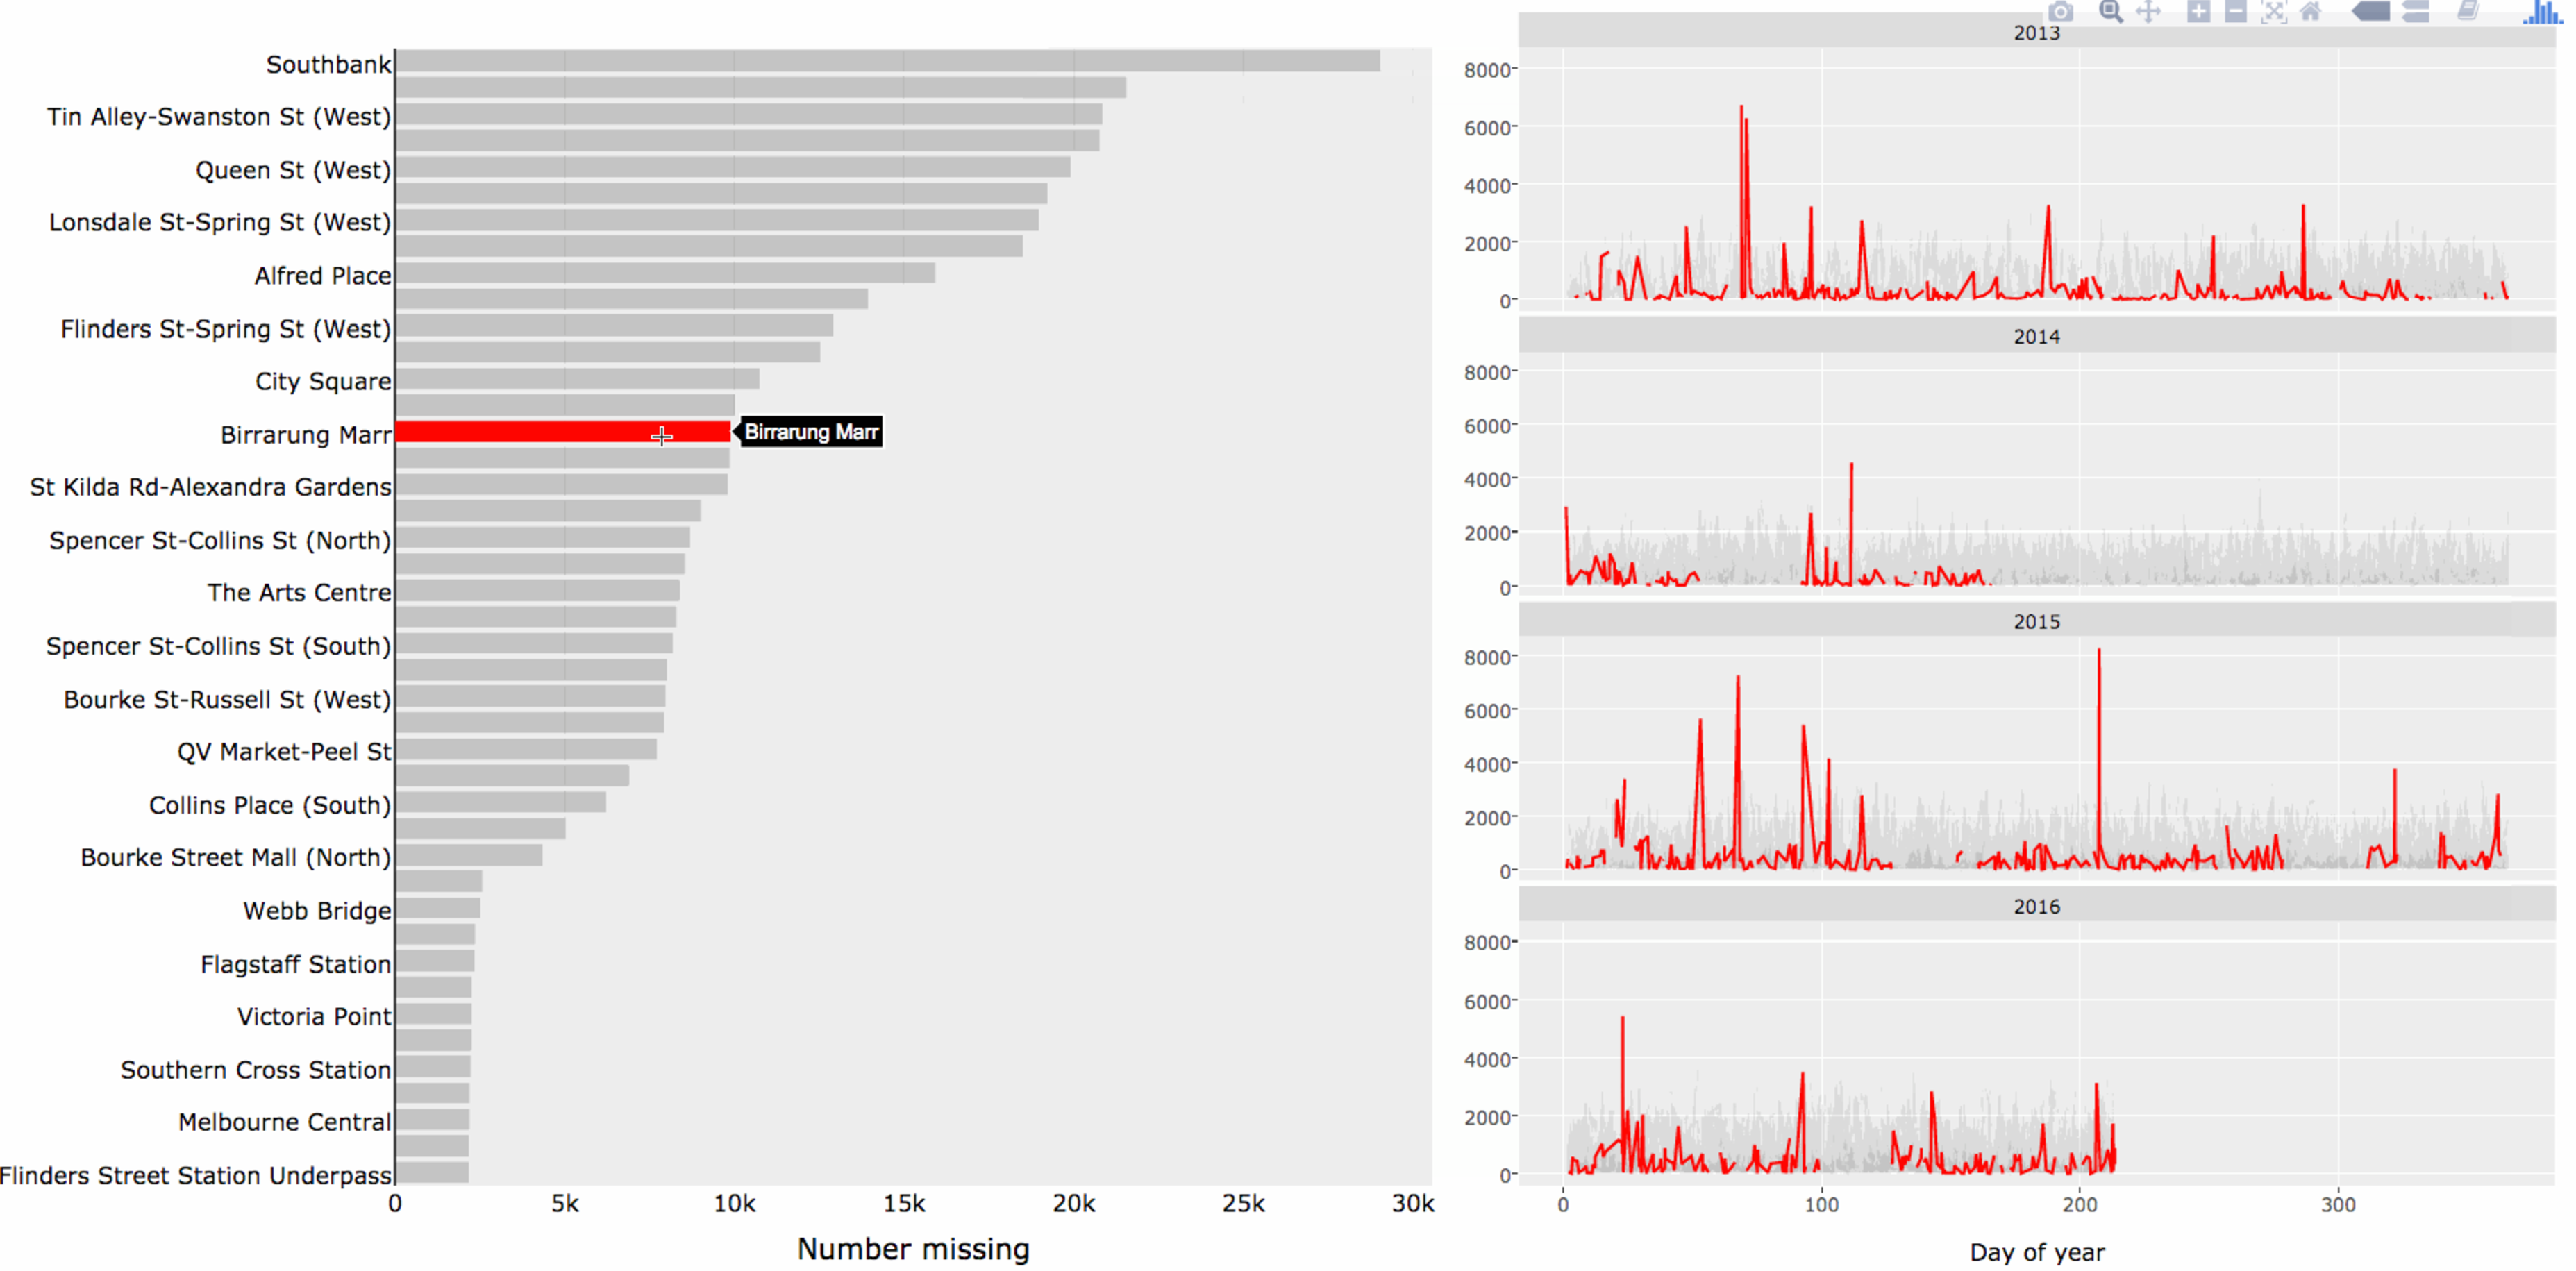
\includegraphics{images/pedestrians-missing.pdf}
\caption{\label{fig:missing-by-time}An interactive bar chart of the number
of missing counts by station linked to a sampled time series of counts.
See \href{https://vimeo.com/189035350}{here} for the corresponding video
and \href{http://cpsievert.github.io/pedestrians/missing-by-time/}{here}
for the interactive figure.}
\end{figure}

\subsubsection{Exploring trend and
seasonality}\label{exploring-trend-and-seasonality}

A time series \(Y_t\) can be thought of as a linear combination of at
least three components:

\[Y_t = T_t + S_t + I_t, \hspace{0.4cm} t \in \{1, \dots, T \} \] where
\(T_t\) is the trend, \(S_t\) is the seasonality, and \(I_t\) is the
``irregular'' component (i.e., remainder). For the sensor data, we could
imagine having multiple types of seasonality (e.g., hour, day, month,
year), but as Figure \ref{fig:missing-by-time} showed, year doesn't seem
to have much effect, and as we will see later, hour of day has a
significant effect (which is sensible for most traffic data), so we
focus on hour of day as a seasonal component. Estimating these
components has important applications in time series modeling (e.g.,
seasonal adjustments), but we could also leverage these estimates to
produce further time series ``features'' to guide our graphical
analysis.

There are many to go about modeling and estimating these time series
components. Partly due to its widespread availability in R, the
\texttt{stl()} function, which is based on LOESS smoothing, is a popular
and reasonable approach (R. B. Cleveland and Terpenning 1990); (R Core
Team 2016). Both the \textbf{anomalous} and \textbf{tscognostics} R
packages use estimates from \texttt{stl()}\footnote{If no seasonal
  component exists, a Generalized Additive Models is used to estimate
  the trend component (Wood 2006).} to measure the strength of trend (as
\(\hat{Var(T_t)}\)) and strength of seasonality (as \(\hat{Var(S_t)}\))
(Hyndman, Wang, and Laptev 2016); (Wang 2016). From these estimates,
they produce other informative summary statistics, such as the seasonal
peak (\(Max_{t}(\hat{S_t})\)), trough (\(Min_{t}(\hat{S_t})\)), spike (
\(Var[(Y_t - \bar{Y})^2]\)); as well as trend linearity
(\(\hat{\beta_1}\)) and curvature (\(\hat{\beta_2}\)) (coefficients from
a 2nd degree polynomial fit to the estimated trend
\(\mu = \beta_0 + \beta_1\hat{T_t} + \beta_2\hat{T_t^2}\)).

Projecting each time series into the 6 dimensional space spanned by
these ``STL features'' allows us to graphically examine the sensor
activity in a reasonable number of interpretable dimensions. Touring is
a graphical technique for viewing such a feature space through
animation. Similar to the rendering and perception of 3D objects in
computer graphics, a tour smoothly interpolates through 2D projections
of numeric variables -- allowing the viewer to perceive the overall
structure and identify clusters and/or outliers (Cook and Swayne 2007).
Figure \ref{fig:pedestrians-tour} shows a couple frames taken from a
tour of random 2D projections -- also known as a grand tour (Asimov
1985). The first frame (the top row) displays a projection with large
weight toward linearity, trough, curvature, and season. From this frame,
it is clear that one sensor (Tin Alley, highlighted in red) is unusual
-- especially along the linearity/curvature/trough dimensions. The
second frame (the bottom row) displays a projection with large weight
towards trend. Along this dimension, another unusual sensor appears
(Bourke St).

\begin{figure}
\centering
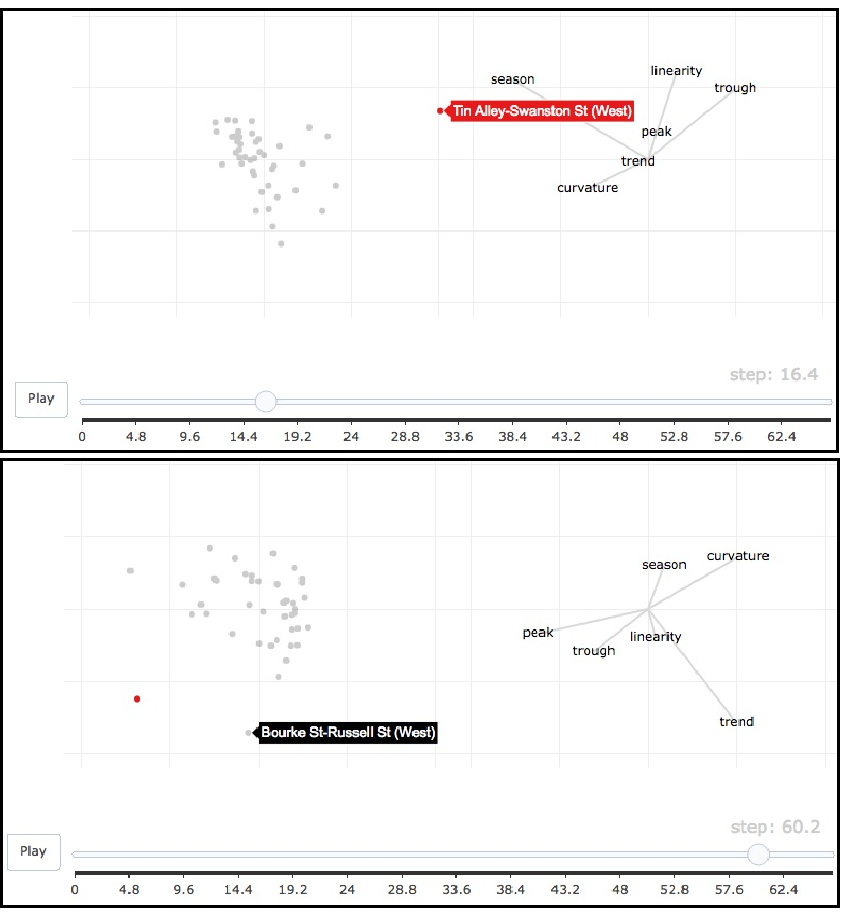
\includegraphics{images/pedestrians-tour.pdf}
\caption{\label{fig:pedestrians-tour}Two frames from a grand tour of
measures generated from seasonal, trend, and irregular time-series
components. The first frame (the top row) displays the state of the tour
roughly 16 seconds into the animation while the second frame (the bottom
row) is at roughly 60 seconds. A given frame displays both a 2D
projection (on the left) and the linear combination of variables used
for the projection (on the right). In both frames, the Tin Alley-Swanson
St (West) sensor is highlighted in red -- a useful technique for
tracking interesting or unusual point(s) throughout a tour.}
\end{figure}

In addition to highlighting observations by painting them directly on
the tour, it can also be useful to link a tour to other views of the
data, such as a parallel coordinates plot. In a parallel coordinates
plot, each observation is represented by a line, and each line
intersects numerous parallel axes (one for each measurement variable)
(Inselberg 1985); (Wegman 1990). Figure \ref{fig:pedestrians-tour-pcp}
links the grand tour from Figure \ref{fig:pedestrians-tour} to a
parallel coordinates plot of the same data, which provides another way
of performing graphical queries (via individual measurements rather than
linear combinations of measurements) (Carr 1996). In a later section, we
leverage this ``linked highlighting'' technique to identify clusters,
but for now, we focus on highlighting unusual sensors.

\begin{figure}
\centering
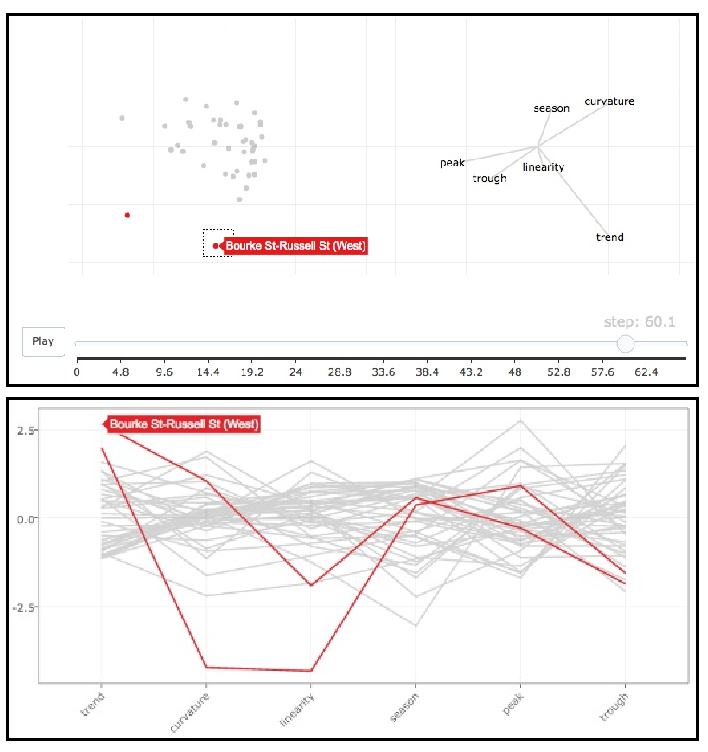
\includegraphics{images/pedestrians-tour-pcp.pdf}
\caption{\label{fig:pedestrians-tour-pcp}Identifying and comparing unusual
sensors (Tin Alley and Swanson St) using linked highlighting between a
grand tour and a parallel coordinates plot. The second frame of Figure
\ref{fig:pedestrians-tour} helped to point out Bourke St as a somewhat
unusual sensor with respect to trend. Highlighting that point and
linking it to a parallel coordinate plot makes it easier to compare
trend across sensors and compare the other measures among sensors of
interest.}
\end{figure}

The appearance of any parallel coordinates plot is effected by at least
two choices -- the ordering of the axes and the scale used to align the
axes. The ordering of axes effects which relationships we end up seeing
-- a \(d\)-dimensional dataset has \(d^2 - \sum_{i=1}^d i\)
relationships, but parallel coordinates can only represent \(d-1\)
relationships at a time. In this case, we have interpretable ``groups''
of variables (trend and seasonality), so Figure
\ref{fig:pedestrians-tour-pcp} uses an ordering to preserve the
grouping. Furthermore, since most of the measurements are roughly
normally distributed, Figure \ref{fig:pedestrians-tour-pcp} centers and
scales each variable to have mean 0 and standard deviation 1. As a
result, it is really obvious that Tin Alley is really unusual with
respect to curvature and linearity, but Bourke St and Tin Alley are only
slightly unusual with respect to trend.

Now that we have a couple sensors of interest, it would help to link to
other views that reveal more details about their sensor activity. Figure
\ref{fig:pedestrians-stl-tour} adds two more linked views to Figure
\ref{fig:pedestrians-tour-pcp}, including the inter-quartile range (IQR)
of counts per hour, and a sample of the raw counts. The former display
is useful for gaining an understanding of the magnitude and variation in
sensor activity (IQR), while the latter is useful for discover outliers
or unusual patterns.\footnote{The same sampling strategy used in Figure
  \ref{fig:missing-by-time} is used to generate the dotplot (count
  versus hour of day).} Highlighting the different sensors with
different colors in each view using a persistent brush fosters
comparison and helps viewers track which graphical markers belong to
which sensor. As a result, it becomes apparent that Tin Alley (in red)
experiences relatively low traffic compared to Bourke St (in blue), and
overall traffic (black).

\begin{figure}
\centering
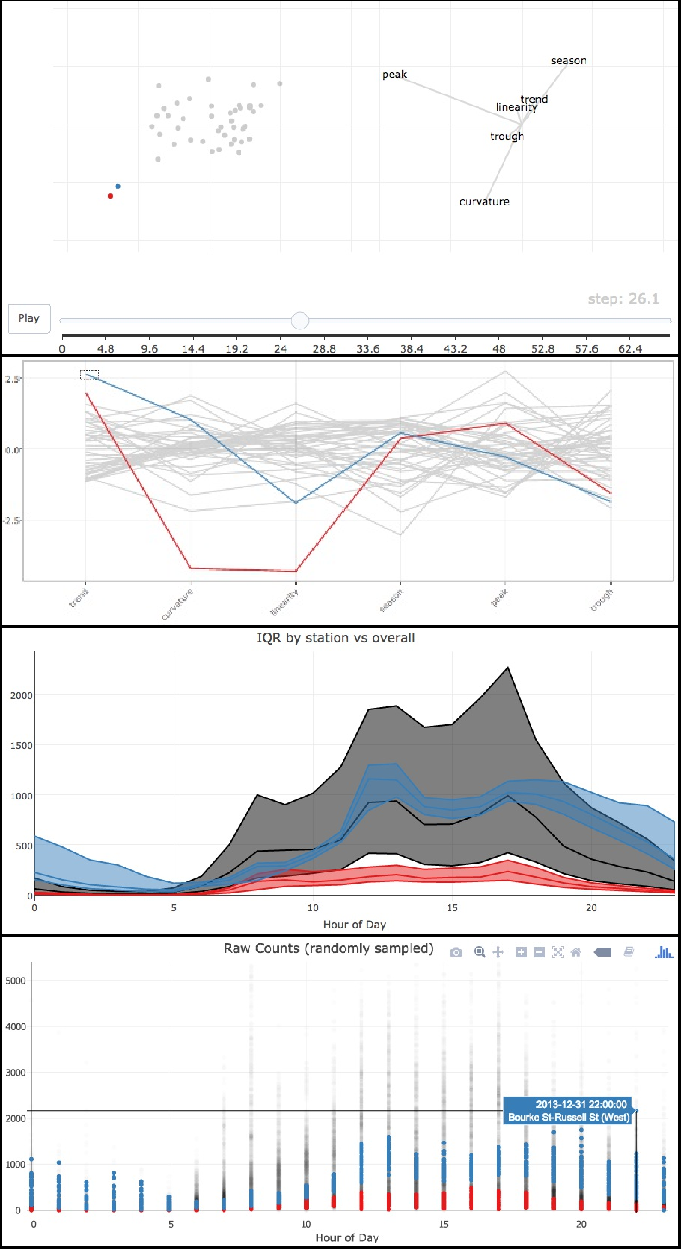
\includegraphics{images/pedestrians-stl-tour.pdf}
\caption{\label{fig:pedestrians-stl-tour}Linking views of seasonal trend
decomposition summaries (first two rows) to the actual time series (last
two rows). By linking raw counts and the hourly IQR, we can see that Tin
Alley (in red) experiences relatively low traffic compared to Bourke St
(in blue), and overall traffic (black). See
\href{https://vimeo.com/192684799}{here} for the corresponding video and
\href{http://cpsievert.github.io/pedestrians/stl-tour/}{here} for the
interactive figure.}
\end{figure}

Hundreds of comparisons and a fair amount of insight could be extracted
from the interactive graphic in Figure \ref{fig:pedestrians-stl-tour},
but focusing just on the STL-based features is somewhat limiting. There
are certainly other features that capture aspects of the time series
that these features have missed. In theory, the mathematics and the
visualization techniques behind Figure \ref{fig:pedestrians-stl-tour}
can be extended to any number of dimensions. In practice, technology and
time typically limits us to tens to hundreds of dimensions. The next
section incorporates more time-series features and also links this
information to a geographic map so we can investigate the relationship
between geographic location and certain features.

\subsubsection{Exploring many features}\label{exploring-many-features}

Figure \ref{fig:pedestrians-cog-tour} is an extension of Figure
\ref{fig:pedestrians-stl-tour} to incorporate 10 other time series
features, as well as a map of Melbourne. In this much larger feature
space, Tin Alley (in red) is still an unusual sensor, but not quite as
unusual as Waterfront City (in blue). Also, rather interestingly, both
of these sensors are located on the outskirts of the city, relative to
the other sensors. It appears Waterfront City is so noticeably unusual
due to its very large value of lumpiness (defined as the variance of
block variances of size 24). Inspecting the unusually high raw counts
for this station reveals some insight as to why that is case -- the
counts are relatively low year-round, but then spike dramatically on new
years eve and on April 13th. A Google search reveals that Waterfront
City is a popular place to watch fireworks. This is a nice example of
how interactive graphics can help us discover and explain \emph{why}
unusual patterns occur.

\begin{figure}
\centering
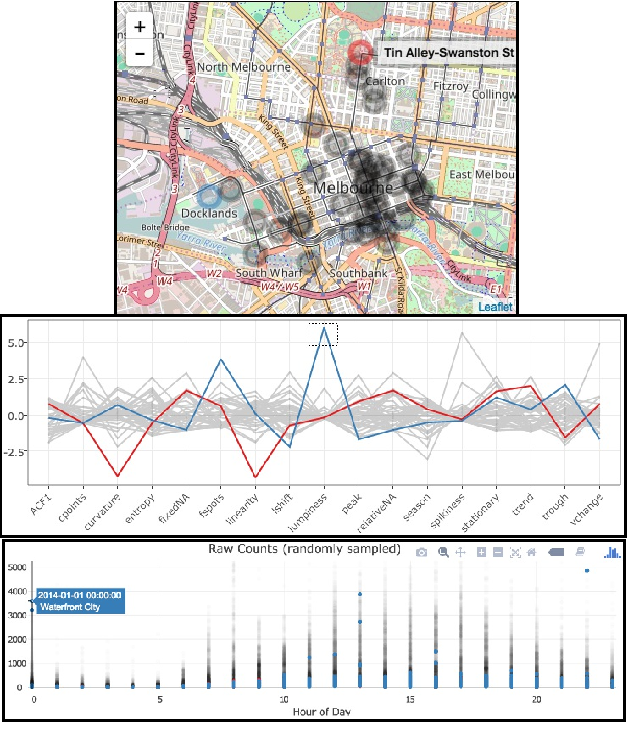
\includegraphics{images/pedestrians-cog-tour.pdf}
\caption{\label{fig:pedestrians-cog-tour}Seventeen time series features
linked to a geographic map as well as raw counts. This static image was
generated using a persistent brush to compare Tin Alley-Swanson St. (in
red) to Waterfront City (in blue). In addition to being unusual in the
feature space, these sensors are also on the outskirts of the city. The
corresponding video and interactive figure (available
\href{https://vimeo.com/192710308}{here} and
\href{http://cpsievert.github.io/pedestrians/cog-tour/}{here}) also
includes a grand tour and raw counts by day of the year.}
\end{figure}

In addition to discovering interesting details, we can use the same
interactive display that generated Figure \ref{fig:pedestrians-cog-tour}
to make meaningful comparisons between groups of sensors. Figure
\ref{fig:pedestrians-cog-tour-acf} uses a persistent linked brush to
compare sensors with a high first order autocorrelation
(\(Corr(Y_t, Y_{t-1})\)), in red, against sensors with low
autocorrelation, in blue. A few interesting observations can be made
from this selection state.

\begin{figure}
\centering
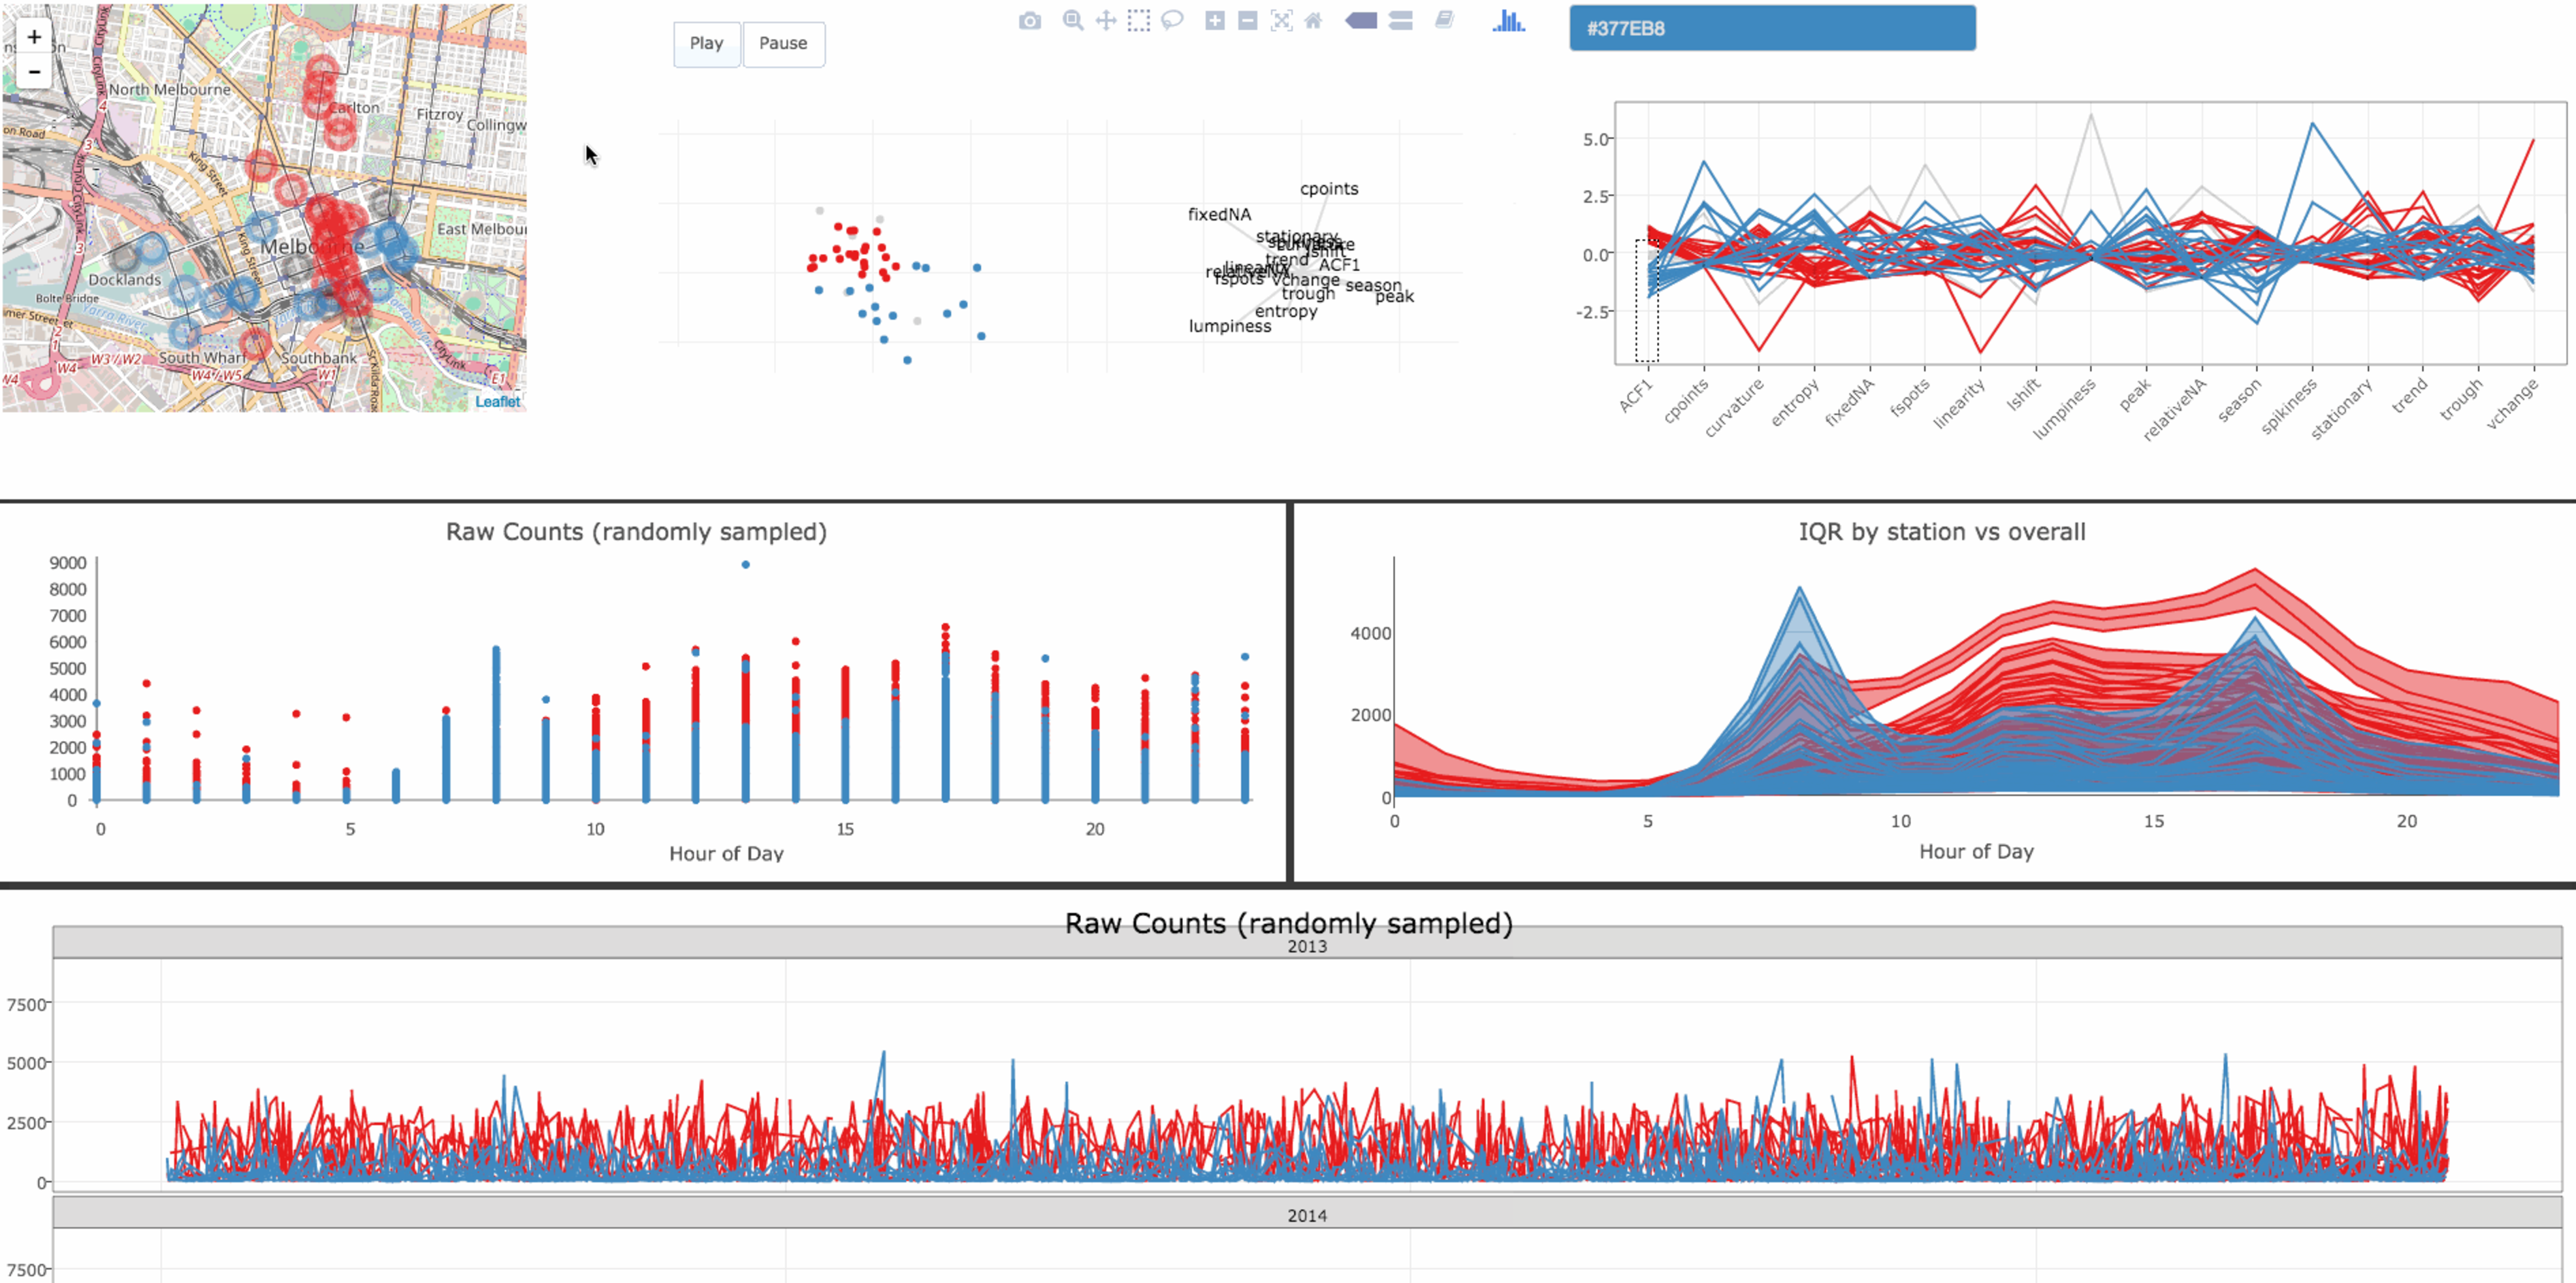
\includegraphics{images/pedestrians-cog-tour-acf.pdf}
\caption{\label{fig:pedestrians-cog-tour-acf}Sensors with high first order
autocorrelation (in red) versus sensors with low autocorrelation (in
blue). See \href{https://vimeo.com/189187319}{here} for the
corresponding video and
\href{http://cpsievert.github.io/pedestrians/cog-tour/}{here} for the
interactive figure.}
\end{figure}

The most striking relationship with respect to autocorrelation in Figure
\ref{fig:pedestrians-cog-tour-acf} is in the geographic locations.
Sensors with high autocorrelation (red) appear along Swanson St. -- the
heart of the central business district in Melbourne. These stations
experience a fairly steady flow of traffic throughout the day since both
tourists and people going to/from work use nearby trains/trams to get
from place to place. On the other hand, sensors with a low
autocorrelation\footnote{It should be noted that the (raw)
  autocorrelation is positive for each station with a minimum of 0.66,
  median of 0.83, and max of 0.94.} see the bulk of their traffic at the
start and end of the work day. It seems that this feature alone would
provide a fairly good criteria for splitting these sensors into 2
groups, which we could verify and study further via hierarchical
clustering.

Figure \ref{fig:pedestrians-dendro} links a dendrogram of a hierarchical
cluster analysis (using the complete linkage method via the
\texttt{hclust()} function in R) to other views of the data. A
persistent brush selects all the sensors under a given node --
effectively providing a tool to choose a number of clusters and
visualize model results in the data space (in real-time). Splitting the
dendrogram at the root node splits the sensors into 2 groups (red and
green) which confirms prior suspicions -- sensors on Swanson St (high
autocorrelation) are most different from sensors on the outskirts of the
city (low autocorrelation). Increasing the number of clusters to 3-4
splits off the unusual sensors that we identified in our previous
observations (Waterfront City, Birrarung Marr, and Tin Alley-Swanson
St).

\begin{figure}
\centering
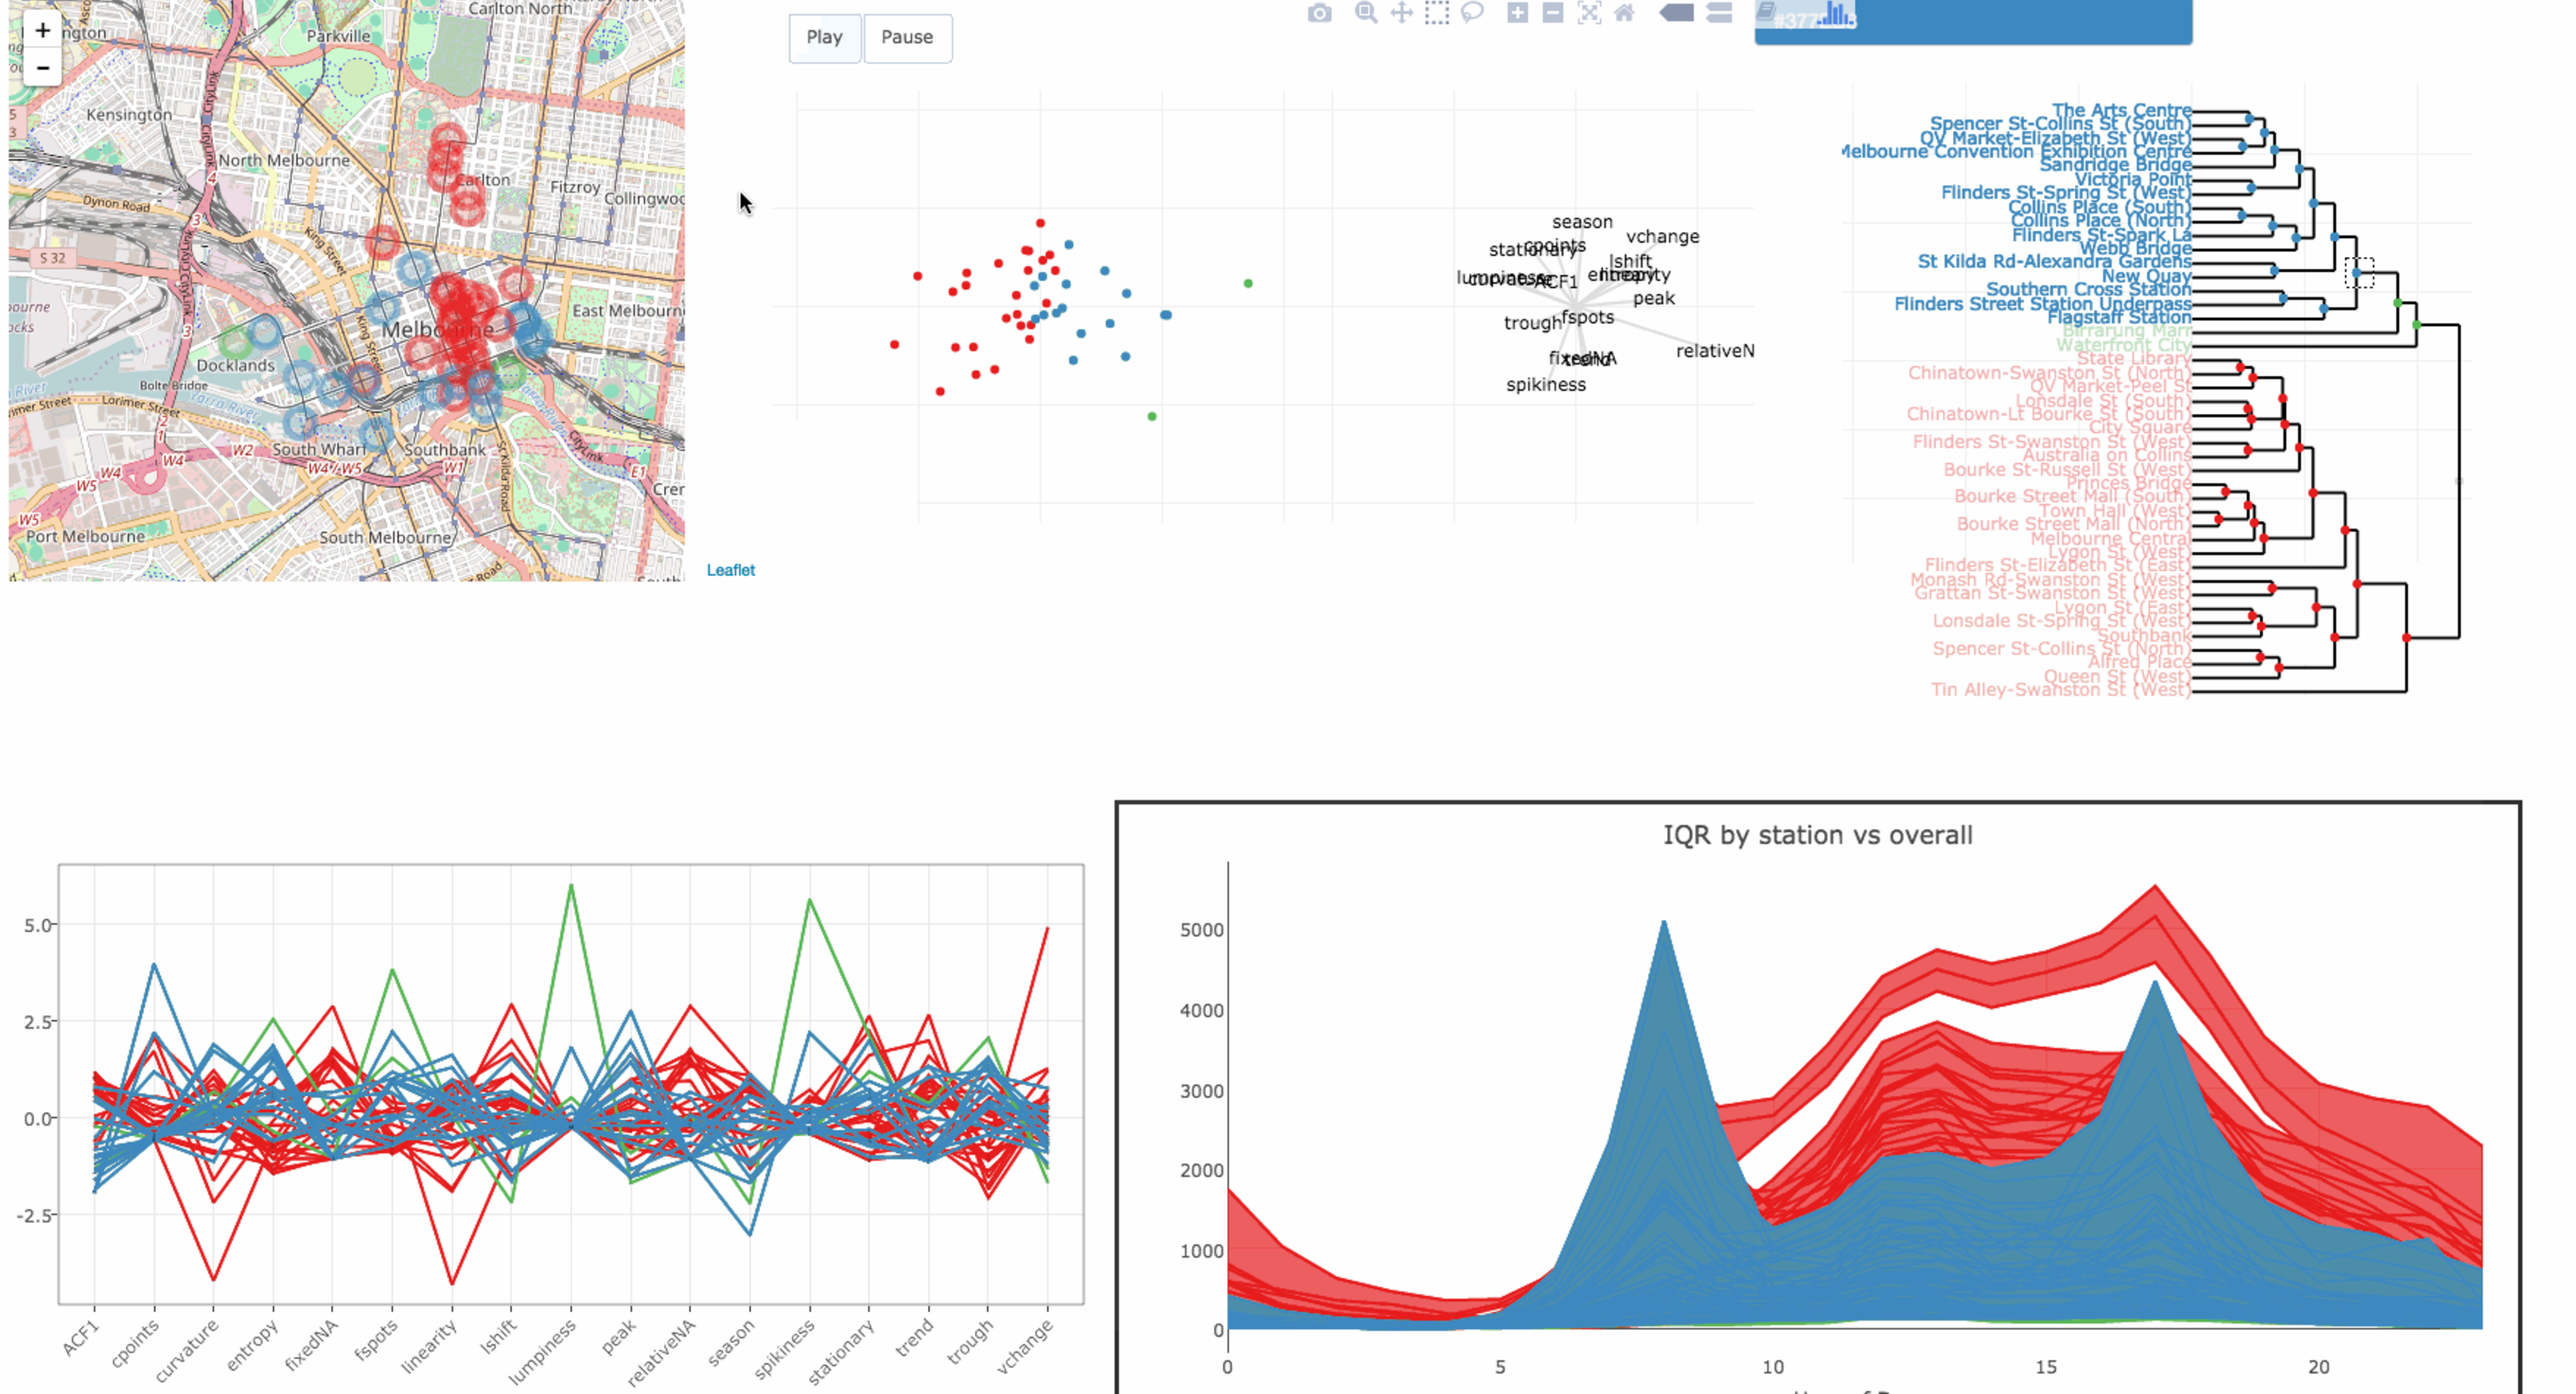
\includegraphics{images/pedestrians-dendro.pdf}
\caption{\label{fig:pedestrians-dendro}Linking a dendrogram of hierarchical
clustering results to multiple views of the raw data. See
\href{https://vimeo.com/189670650}{here} for the corresponding video and
\href{http://cpsievert.github.io/pedestrians/tour-dendro/}{here} for the
interactive figure.}
\end{figure}

This case study on pedestrian counts uses interactive graphic techniques
for numerous data analysis tasks. In fact, Figure
\ref{fig:pedestrians-cog-tour} alone provides at least one example of
each task outlined by Cook, Buja, and Swayne (1996): finding Gestalt,
posing queries, and making comparisons. Furthermore, as Figure
\ref{fig:pedestrians-cog-tour} shows, and Wickham, Cook, and Hofmann
(2015) writes, these same interactive techniques can also be a helpful
for understanding, inspecting, and diagnosing statistics models. The
next case study on Zika virus infections demonstrates how interactive
graphics can be useful for tracking disease outbreak and detecting data
quality issues.

\hypertarget{tracking-disease-outbreak}{\subsection{Tracking disease
outbreak}\label{tracking-disease-outbreak}}

The next case study investigates Zika disease outbreaks across North,
Central, and South America. The data was obtained from a publically
available repository that curates data from numerous public reports
across numerous countries and regions (Rodriguez et al. 2016). Of
course, each country has a different reporting method, so reported cases
can and do fall under many different categories. Thankfully, Rodriguez
et al. (2016) have done the tedious work of standardizing these codes so
we can combine all of these reports into a single dataset. In some
countries, reports are broken down to by different demographics, and
include reports of similar diseases such as Flavi virus and GBS, but
this analysis focuses specifically on suspected/confirmed Zika cases at
the location level.

The R package \textbf{zikar} bundles suspected/confirmed Zika cases at
the location level and provides specially designed tools for visualizing
it (Sievert 2016c). All the graphics in this section were generated via
the \texttt{explore()} function from \textbf{zikar}, which invokes a
\textbf{shiny} app with linked interactive graphics (Chang et al.
2015).\footnote{A hosted version of this web application is avaliable
  \href{http://104.131.111.111:3838/zikar/}{here}.} Figure
\ref{fig:zikar} displays the default view of the web application, which
provides a concise overview of the reported counts. The map on the
left-hand side shows the different reporting locations. The non-black
markers represent multiple locations, and hovering over a marker reveals
the entire region that the marker represents. From this, we can see that
the bulk of reporting locations are in the northern part of South
America and the southern part of Central America. The right hand side of
Figure \ref{fig:zikar} shows the overall density of weekly cases (on a
log scale) as well as the weekly median over time.

\begin{figure}
\centering
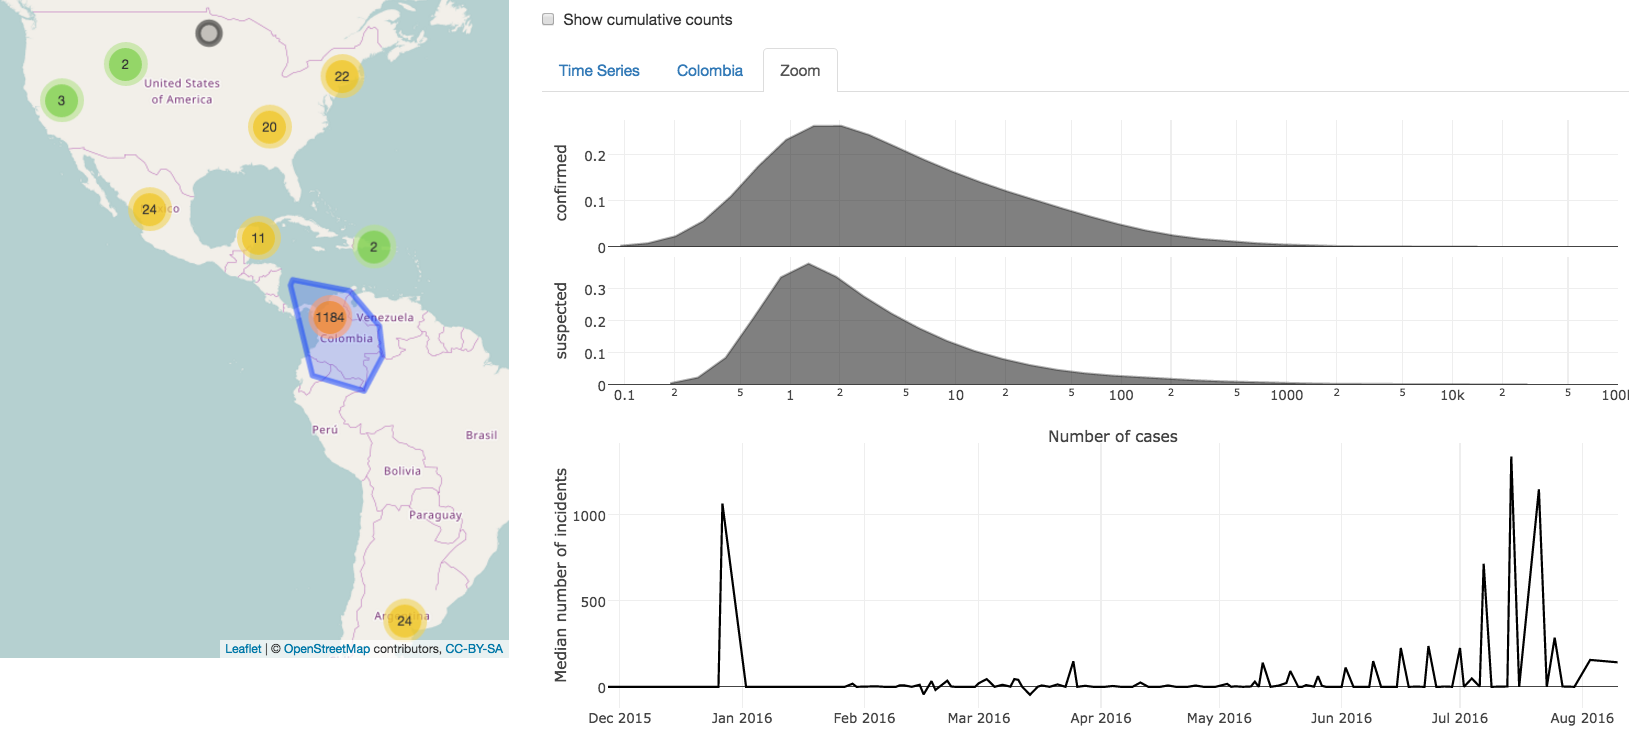
\includegraphics{images/zikar}
\caption{\label{fig:zikar}Multiple views of the Zika outbreak data. On the
left-hand side is a map of the reporting locations. On the right is the
overall density of suspected/confirmed cases reported per week (on a log
scale), and the overall weekly median over time.}
\end{figure}

Zooming and panning to a particular region on the interactive map
reveals more information conditioned on the bounding box of the map.
Figure \ref{fig:zikar-zoom} displays information specific to the
Dominican Republic. In the map itself, the ``marker clusters'' have
updated for a more granular view of the number of locations reporting
within the area. In the other views, statistics conditional upon this
region (in red) are overlaid against overall statistics (in black) for
fast and easy comparison(s). Figure \ref{fig:zikar-zoom} shows the
density of suspected cases in the Dominican is much higher than the
overall density, and the density for confirmed cases has a much larger
amount of variation. Furthermore, the weekly median within this region
is consistently higher from March 2016 to July 2016.

\begin{figure}
\centering
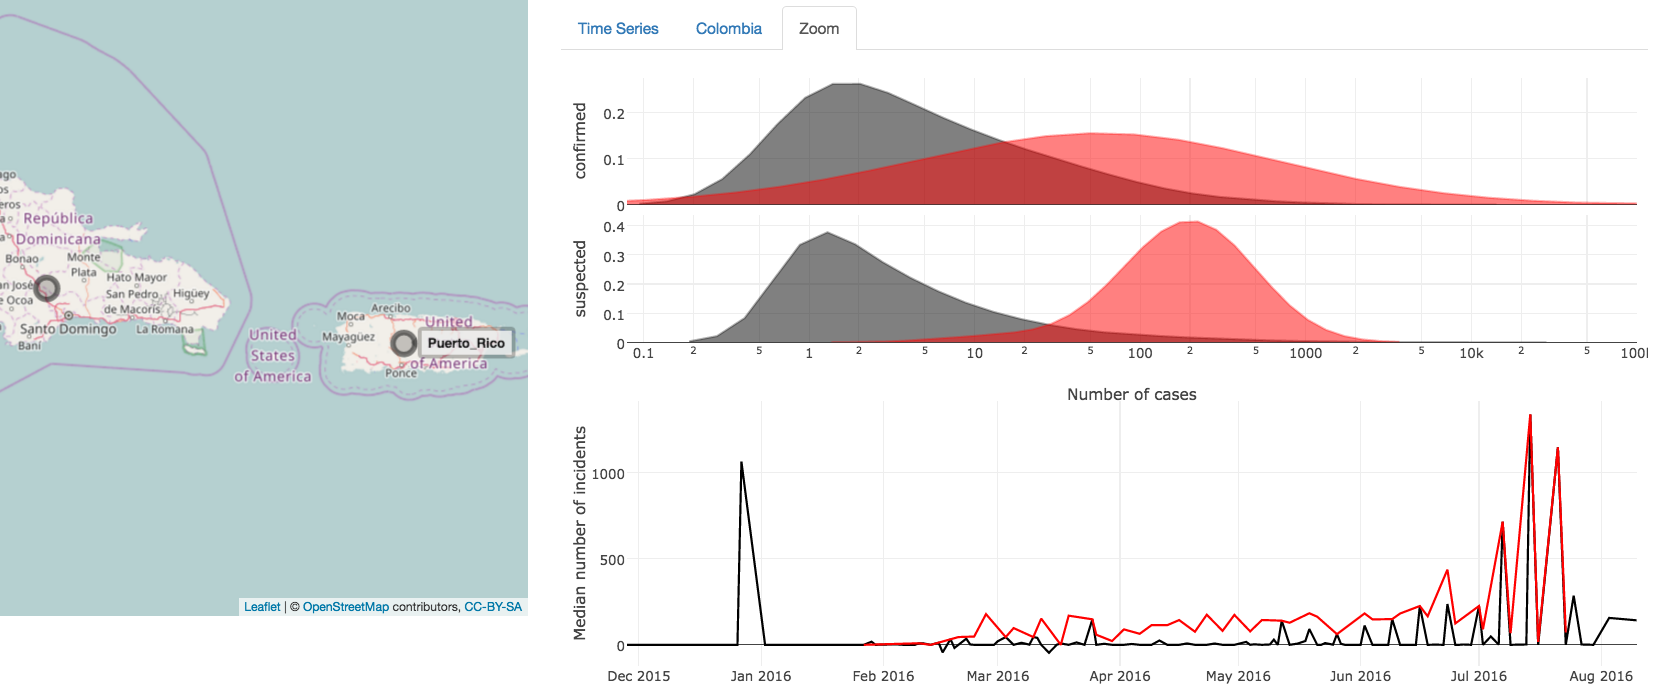
\includegraphics{images/zikar-zoom}
\caption{\label{fig:zikar-zoom}A comparison of the overall cases (in black)
to the cases conditional on the map bounds (in red). Zooming and panning
the interactive map dynamically updates the density estimates and median
number of incidents.}
\end{figure}

Figure \ref{fig:zikar} helps to point out an issue with the data -- in
some weeks, the median number of all reported cases is negative. Using
the zooming and panning capabilities of Figure \ref{fig:zikar}, one may
quickly find a sub-region of the map that reflects the same overall
issue, which helps to guide an investigation into why this issue exists.
Figure \ref{fig:zikar-nicaragua} uses this functionality to find that
both El Salvador and Nicaragua report negative counts, at different
times of the year. Considering that these countries report a cumulative
count of currently infected people, these negative non-cumulative counts
indicate mis-diagnosis or death. Since deaths caused by Zika in adults
are quite rare, and symptoms from the Zika virus are hard to
differentiate from the more common Dengue virus (another disease spread
via infected mosquitoes), mis-diagnosis seems to be the more likely
reason for the negative counts (McNeil and Victor 2016).

\begin{figure}
\centering
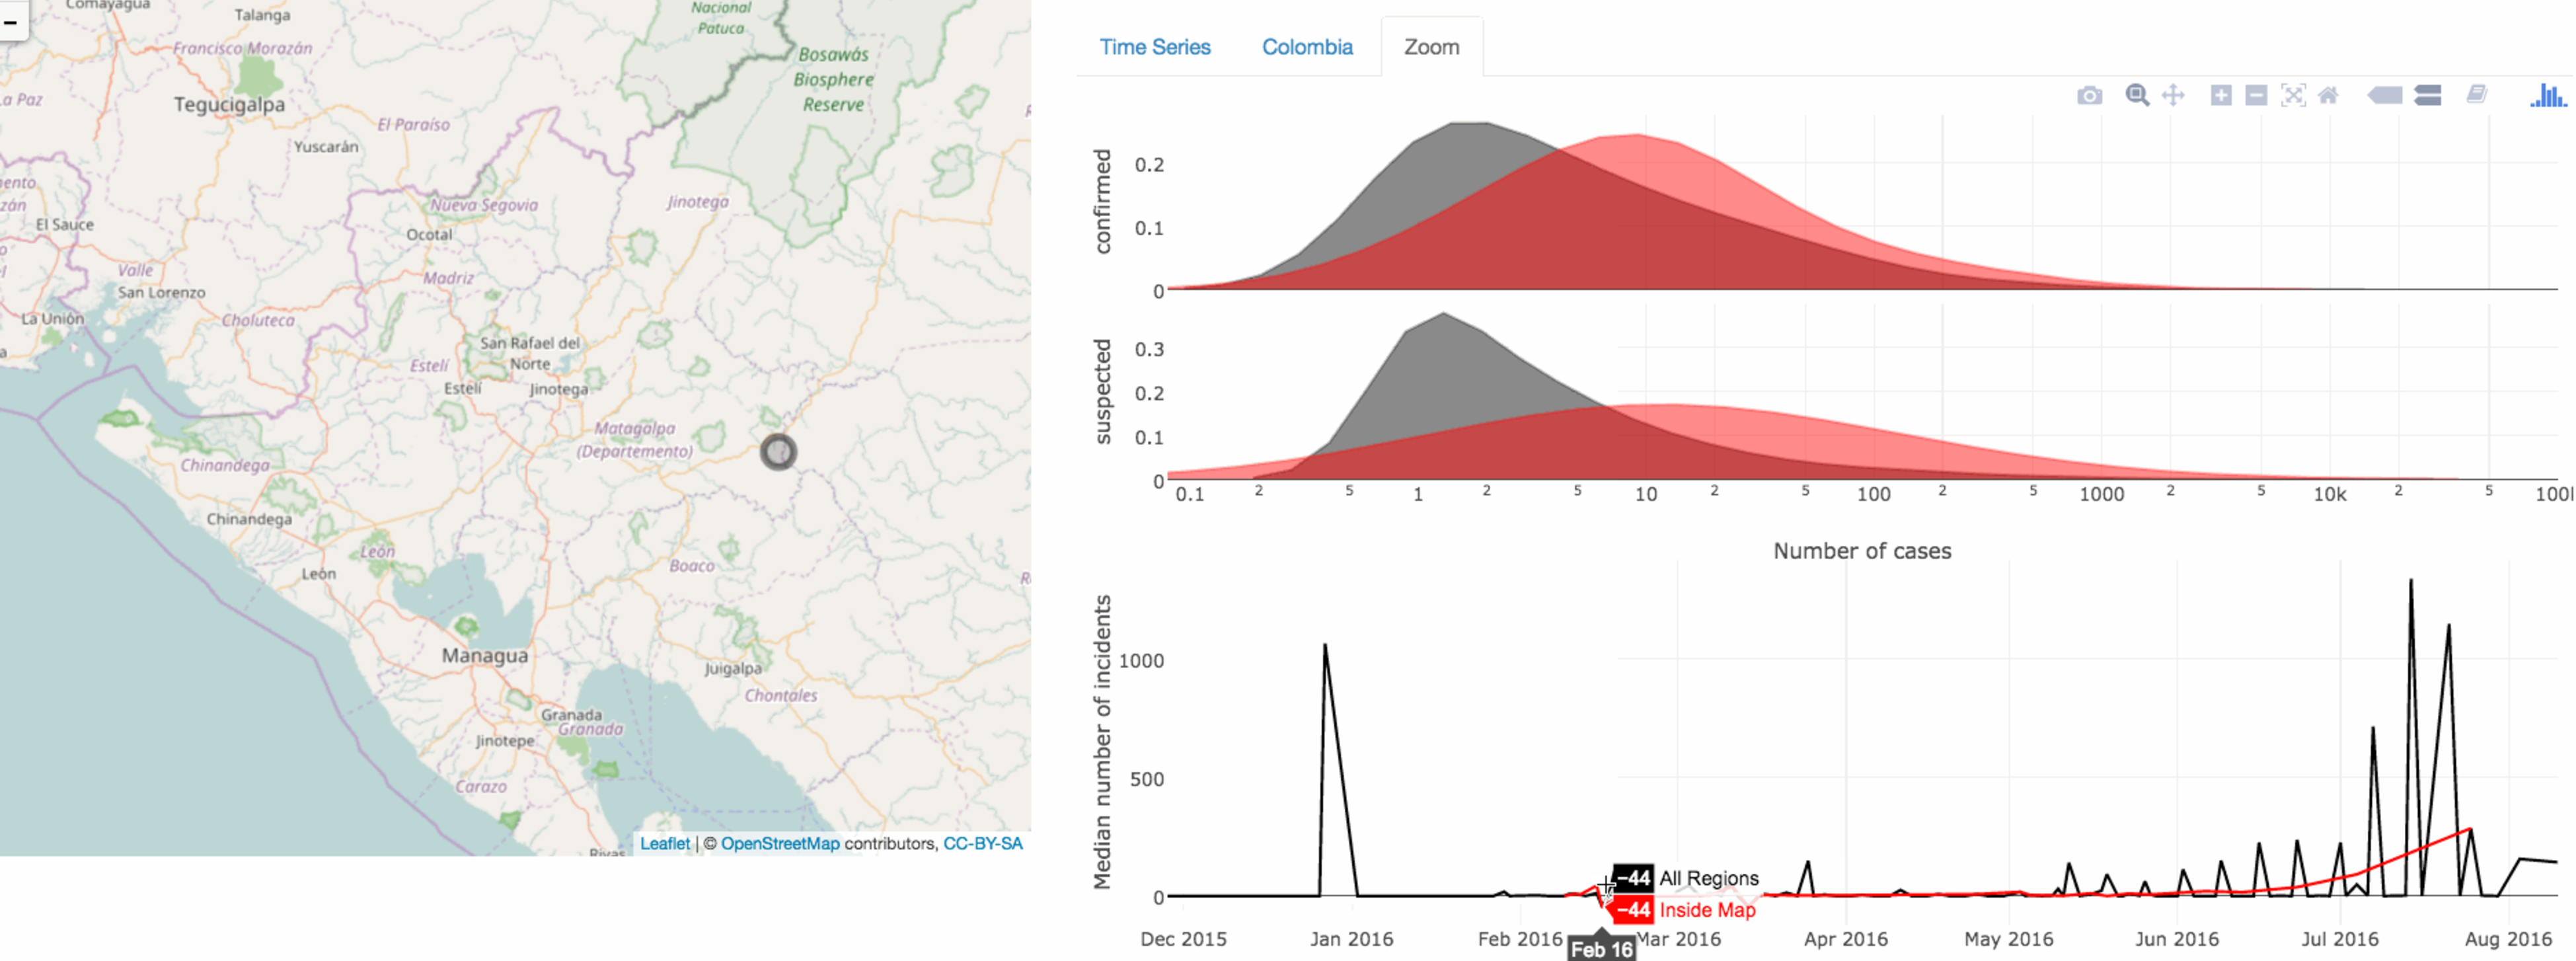
\includegraphics{images/zikar-nicaragua.pdf}
\caption{\label{fig:zikar-nicaragua}Zooming and panning to a region of the
map that has a negative median of overall cases (Nicaragua). A video of
the zooming and panning may be viewed
\href{https://vimeo.com/190610577}{here}.}
\end{figure}

As it turns out, Nicaragua and El Salvador are not the only countries
that have reported a lower cumulative count from one week to the next.
Figure \ref{fig:zikar-cumulative} shows cumulative confirmed (in red)
and suspected (in blue) counts by location within 9 different countries.
Argentina is another country that has clearly encountered mis-diagnosis
issues -- there is a consistent dip in counts across all locations
within the country on two particular dates in May 2016. Although Figure
\ref{fig:zikar-cumulative} covers almost all the countries in this data,
it only covers \textasciitilde{}5\% of all reporting locations. Colombia
alone accounts for \textasciitilde{}95\% of all locations found in this
data and has some unique reporting issues of its own.

\begin{figure}
\centering
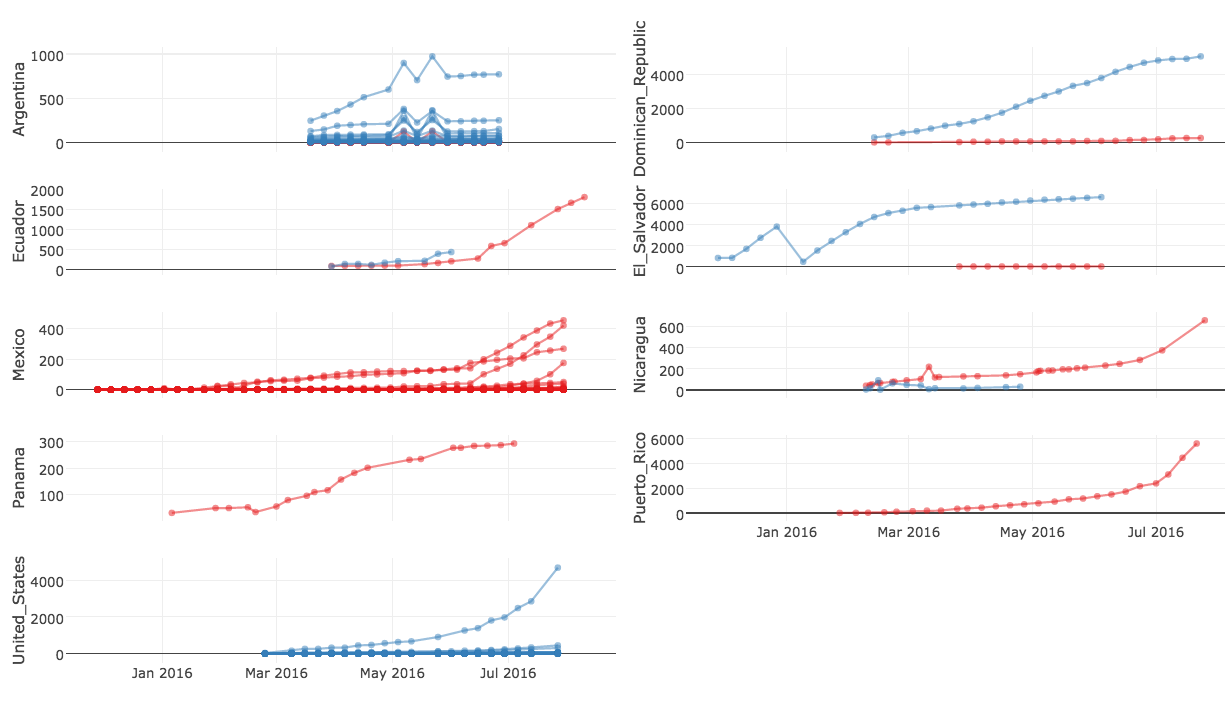
\includegraphics{images/zikar-cumulative}
\caption{\label{fig:zikar-cumulative}Cumulative confirmed (in red) and
suspected (in blue) counts by location within 9 different countries.}
\end{figure}

Figure \ref{fig:zikar-colombia} shows the cumulative number of confirmed
(in red) and suspected (in blue) cases for every reporting location in
Colombia. From the static version of Figure \ref{fig:zikar-colombia}, it
seems plausible that every location re-classified all confirmed cases to
suspected around mid-March. By clicking on a particular line (shown in
the video of Figure \ref{fig:zikar-colombia}) to highlight the
confirmed/suspected counts for a particular location, it becomes even
more obvious that every Colombian location simply changed all their
cases from confirmed to suspected.

\begin{figure}
\centering
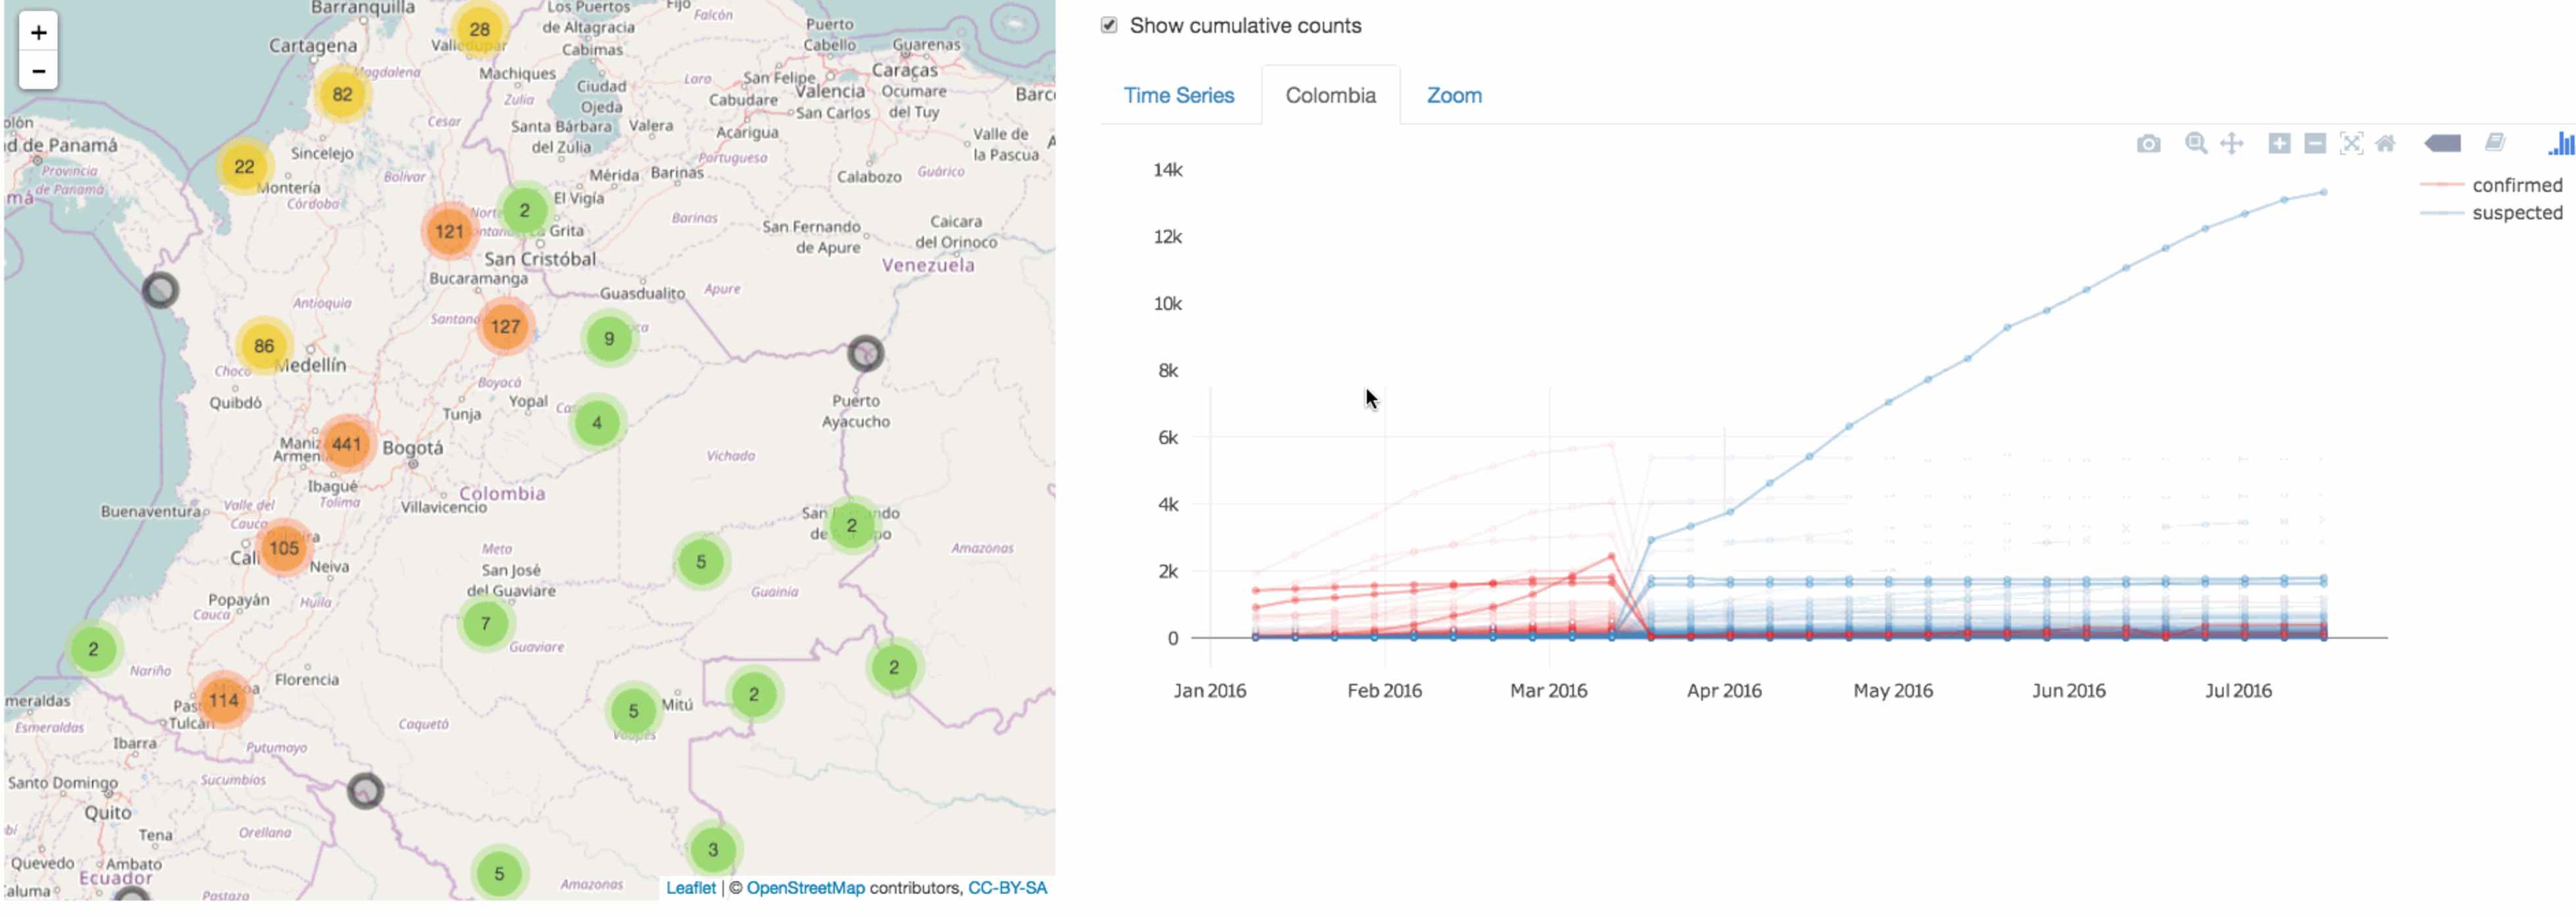
\includegraphics{images/zikar-colombia.pdf}
\caption{\label{fig:zikar-colombia}Highlighting cumulative confirmed (in
red) and suspected (in blue) counts by location within Colombia to
verify re-classifications from confirmed to suspected. A video of the
interactive highlighting may be viewed
\href{https://vimeo.com/190736801}{here}.}
\end{figure}

This case study shows how interactive graphics can be useful to discover
issues in data that should be addressed before any statistical modeling
occurs. For this reason, they are particularly useful for analysts
coming at the problem with a lack of domain expertise, and can provide
insight helpful for downstream analysis. The next case study uses
interactive graphics to explore Australian election data and provides a
nice example of combining numerous data sources into a single dashboard
of linked views.

\hypertarget{exploring-australian-election-data}{\subsection{Exploring
Australian election data}\label{exploring-australian-election-data}}

The next case study takes a look at the relationship between
demographics and voting behavior in the 2013 Australian general
election. Demographic information was obtained from the Australian
Bureau of Statistics (ABS)\footnote{Downloaded from
  \url{https://www.censusdata.abs.gov.au/datapacks/}}, voting
information was obtained from the Australian Electoral Commission
(AEC)\footnote{Downloaded from
  \url{http://www.aec.gov.au/elections/federal_elections/2013/downloads.htm}},
and all the data as well as the interactive graphics presented here are
available via the R package \textbf{eechidna} (Cook et al. 2016).
Thankfully, these data sources can be linked via electoral boundaries
from the 2013 election (and the geo-spatial boundaries are also
available\footnote{\url{http://www.aec.gov.au/Electorates/gis/gis_datadownload.htm}}),
making it possible to explore the relationship between voting behavior
and demographics across electorates.

Figure \ref{fig:eechidna-2p} shows demographics of electorates that
elected candidates (for the House of Representatives in the 2013 general
election) from the Liberal Party in green, the Australian Labor Party in
orange, and all other parties in black. As shown in
\href{https://vimeo.com/191553616}{this video}, Figure
\ref{fig:eechidna-2p} was generated via the \texttt{launchApp()}
function from \textbf{eechidna}, which invokes an interactive
visualization where electorates may be graphically queried according to
voting outcomes, geography, and/or demographics. To foster comparisons,
density estimates for all the 32 different demographics are displayed by
default, but the number of demographics may also be restricted when
invoking \texttt{launchApp()}.

\begin{figure}
\centering
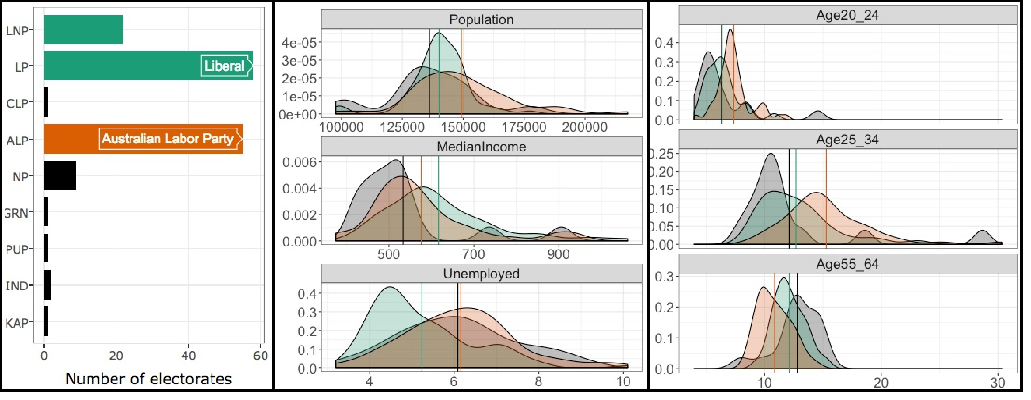
\includegraphics{images/eechidna-2p.pdf}
\caption{\label{fig:eechidna-2p}Electorate demographics among the Liberal
Party (in green), the Australian Labor Party (in orange), and other
parties (in black). The vertical lines represent the mean value within
each group. The interactive application used to generate this image may
be accessed \href{http://104.131.111.111:3838/eechidna/}{here} and a
video of the interactive highlighting may be viewed
\href{https://vimeo.com/191553616}{here}.}
\end{figure}

The density estimates in the lower portion of Figure
\ref{fig:eechidna-2p} suggest that Labor electorates tend to be younger
(in particular, they have a higher percentage of 20-34 year olds, and
lower percentage of 55-64), are more unemployed, have lower income, and
are more populated. Most of these characteristics are not surprising
given the ideologies of each party; however, it is surprising to see a
relationship between the population within electorate and the elected
party. In theory, electorates should be divided roughly equally with
respect to population so that a single vote in one electorate counts as
much as a vote in another electorate. However, in practice, there has to
be some variation in population; and as it turns out, more populated
electorates tend to vote Labor, implying that (on average) a vote
towards the Labor party counts less than a vote for the Liberal party.

Figure \ref{fig:eechidna-2p} was created by painting the relevant bars
in the upper-left hand panel of Figure \ref{fig:eechidna-2p-2}. Note
that, due to the similarities of the parties, both the Liberal National
Party of Queensland (LNP) and the Liberal Party are grouped into a
single liberal party (colored in green). The interaction with the bar
chart not only populates relevant density estimates, as in Figure
\ref{fig:eechidna-2p}, but it also colors every graphical mark
representing the corresponding electorates in the other views shown in
Figure \ref{fig:eechidna-2p-2}.

The line chart in the upper-right hand panel of Figure
\ref{fig:eechidna-2p-2} shows the proportion of 1st preference votes for
each party within a given electorate -- showing an expected difference
between ALP/LP/LNP voting as well as other interesting patterns
(e.g.~liberal party electorates tend to have a higher proportion of 1st
preference votes going to the PUP party). The left-hand panel of Figure
\ref{fig:eechidna-2p-2} displays the absolute difference in vote totals
within electorates, making it easy to identify closely contested
electorates (more on this later). The right-hand panel of Figure
\ref{fig:eechidna-2p-2} displays a map of Australia with polygons
outlining the electorate boundaries. Since the boundaries within highly
populated areas (e.g., Melbourne, Sydney, and Brisbane) are so small,
the location of points (on top of the map) were adjusted by a force
layout algorithm in order to avoid too much overplotting.

\begin{figure}
\centering
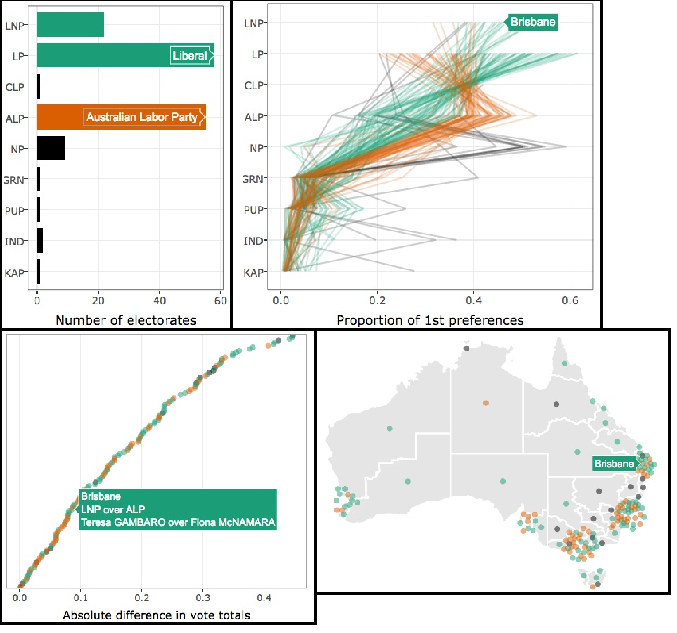
\includegraphics{images/eechidna-2p-2.pdf}
\caption{\label{fig:eechidna-2p-2}Comparing voting outcomes and geographic
location among the Liberal Party (in green), the Australian Labor Party
(in orange), and other parties (in black). The bar chart in the
upper-left hand panel shows the number of electorates won by each party.
The upper-right hand panel shows the proportion of 1st preference votes
for each party for given electorate. The lower-left hand panel shows the
absolute difference in vote totals for each electorate. The lower-right
hand panel show the locations of electorates.}
\end{figure}

Although interaction with the bar chart in Figure
\ref{fig:eechidna-2p-2} helped to generate Figures \ref{fig:eechidna-2p}
and \ref{fig:eechidna-2p-2}, electorates may be queried via directly
manipulation with any of these plots. For example, Figure
\ref{fig:eechidna-diff} was generated by brushing the electorates that
were determined by less than 10\% of the vote total (via the plot with
the absolute difference in vote totals).

\begin{figure}
\centering
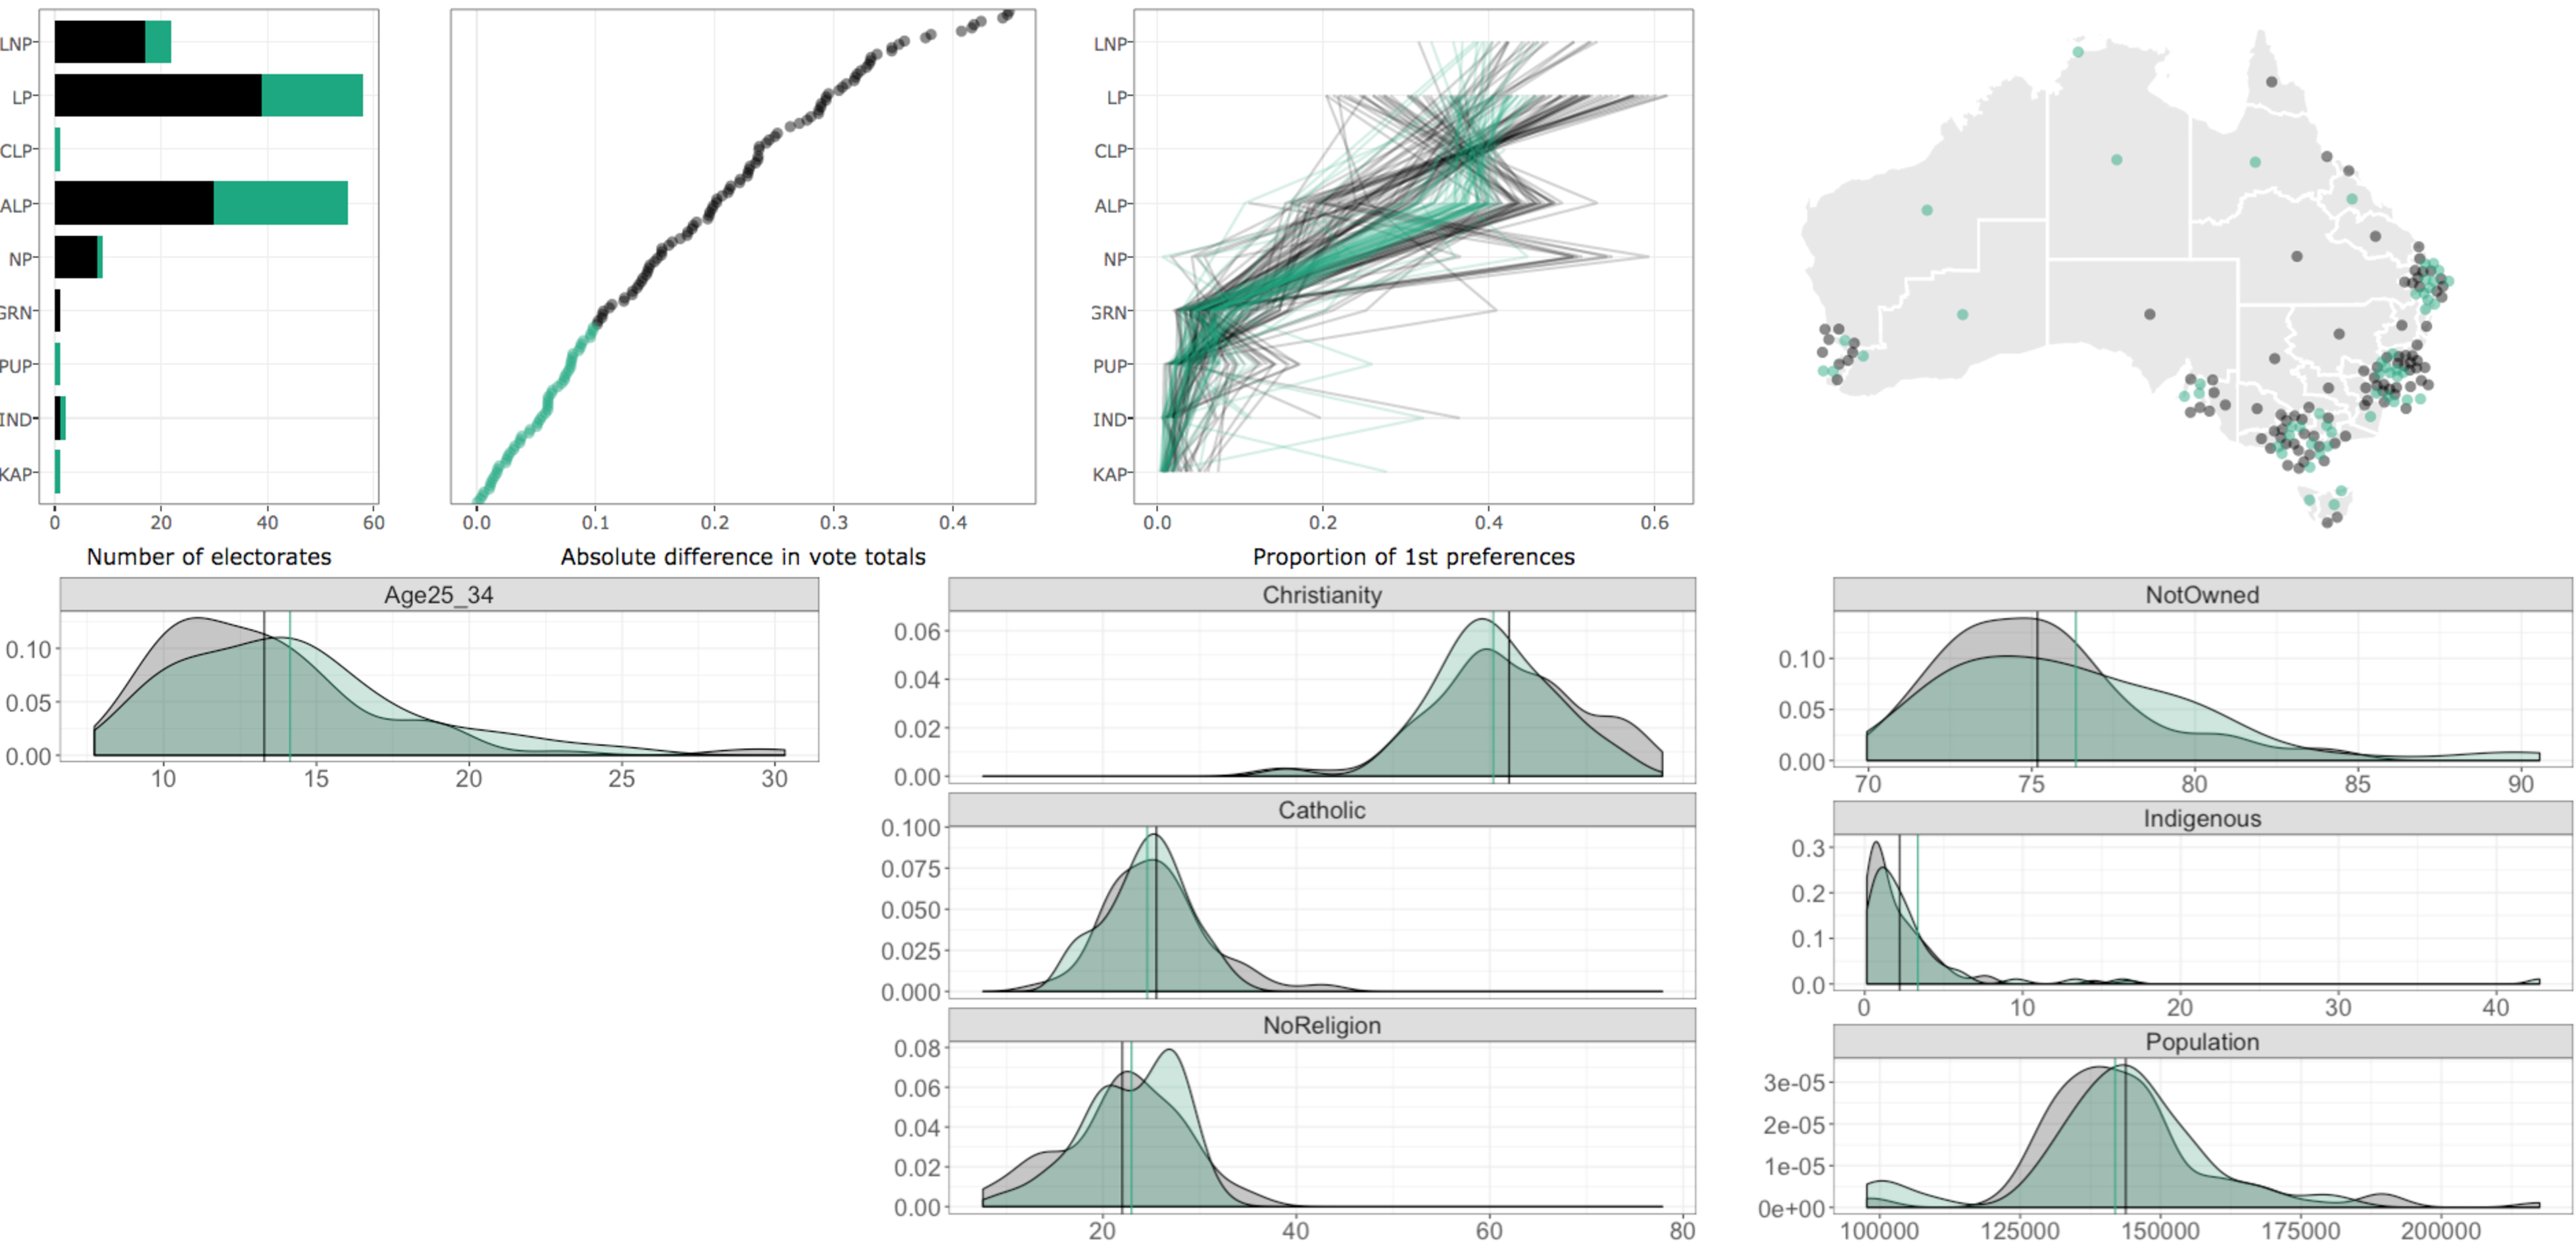
\includegraphics{images/eechidna-diff.pdf}
\caption{\label{fig:eechidna-diff}Electorates that were determined by less
than 10 percent of the total vote. These electorates tend to have voters
that are younger, less religious, are less likely to own property, and
lean towards the Labor party.}
\end{figure}

Figure \ref{fig:eechidna-diff} highlights closely contested electorates
(determined by less than 10\% of the vote total) which provides insight
into the demographics of voters that future political campaigns should
target in order to maximize their campaigning efforts. Voters in these
competitive areas tend to have a high proportion of 25-34 year olds,
have more diverse religious backgrounds, are less likely to own
property, and a higher percentage of the population are Indigenous.
Unsurprisingly, these electorates lean towards the Labor party, but
there are a few electorates within this group that have a surprising
population (around the minimum of 100,000 people). Figure
\ref{fig:eechidna-diff2} paints electorates with a population around the
minimum orange, which reveals a striking geographic relationship among
these electorates -- almost all of them are in Tasmania (with the
exception of one in the Northern Territory). Furthermore, as
\ref{fig:eechidna-diff2} shows, all of these electorates (except for
Denison), experienced a close election, so campaign efforts would be
well spent in these electorates.

\begin{figure}
\centering
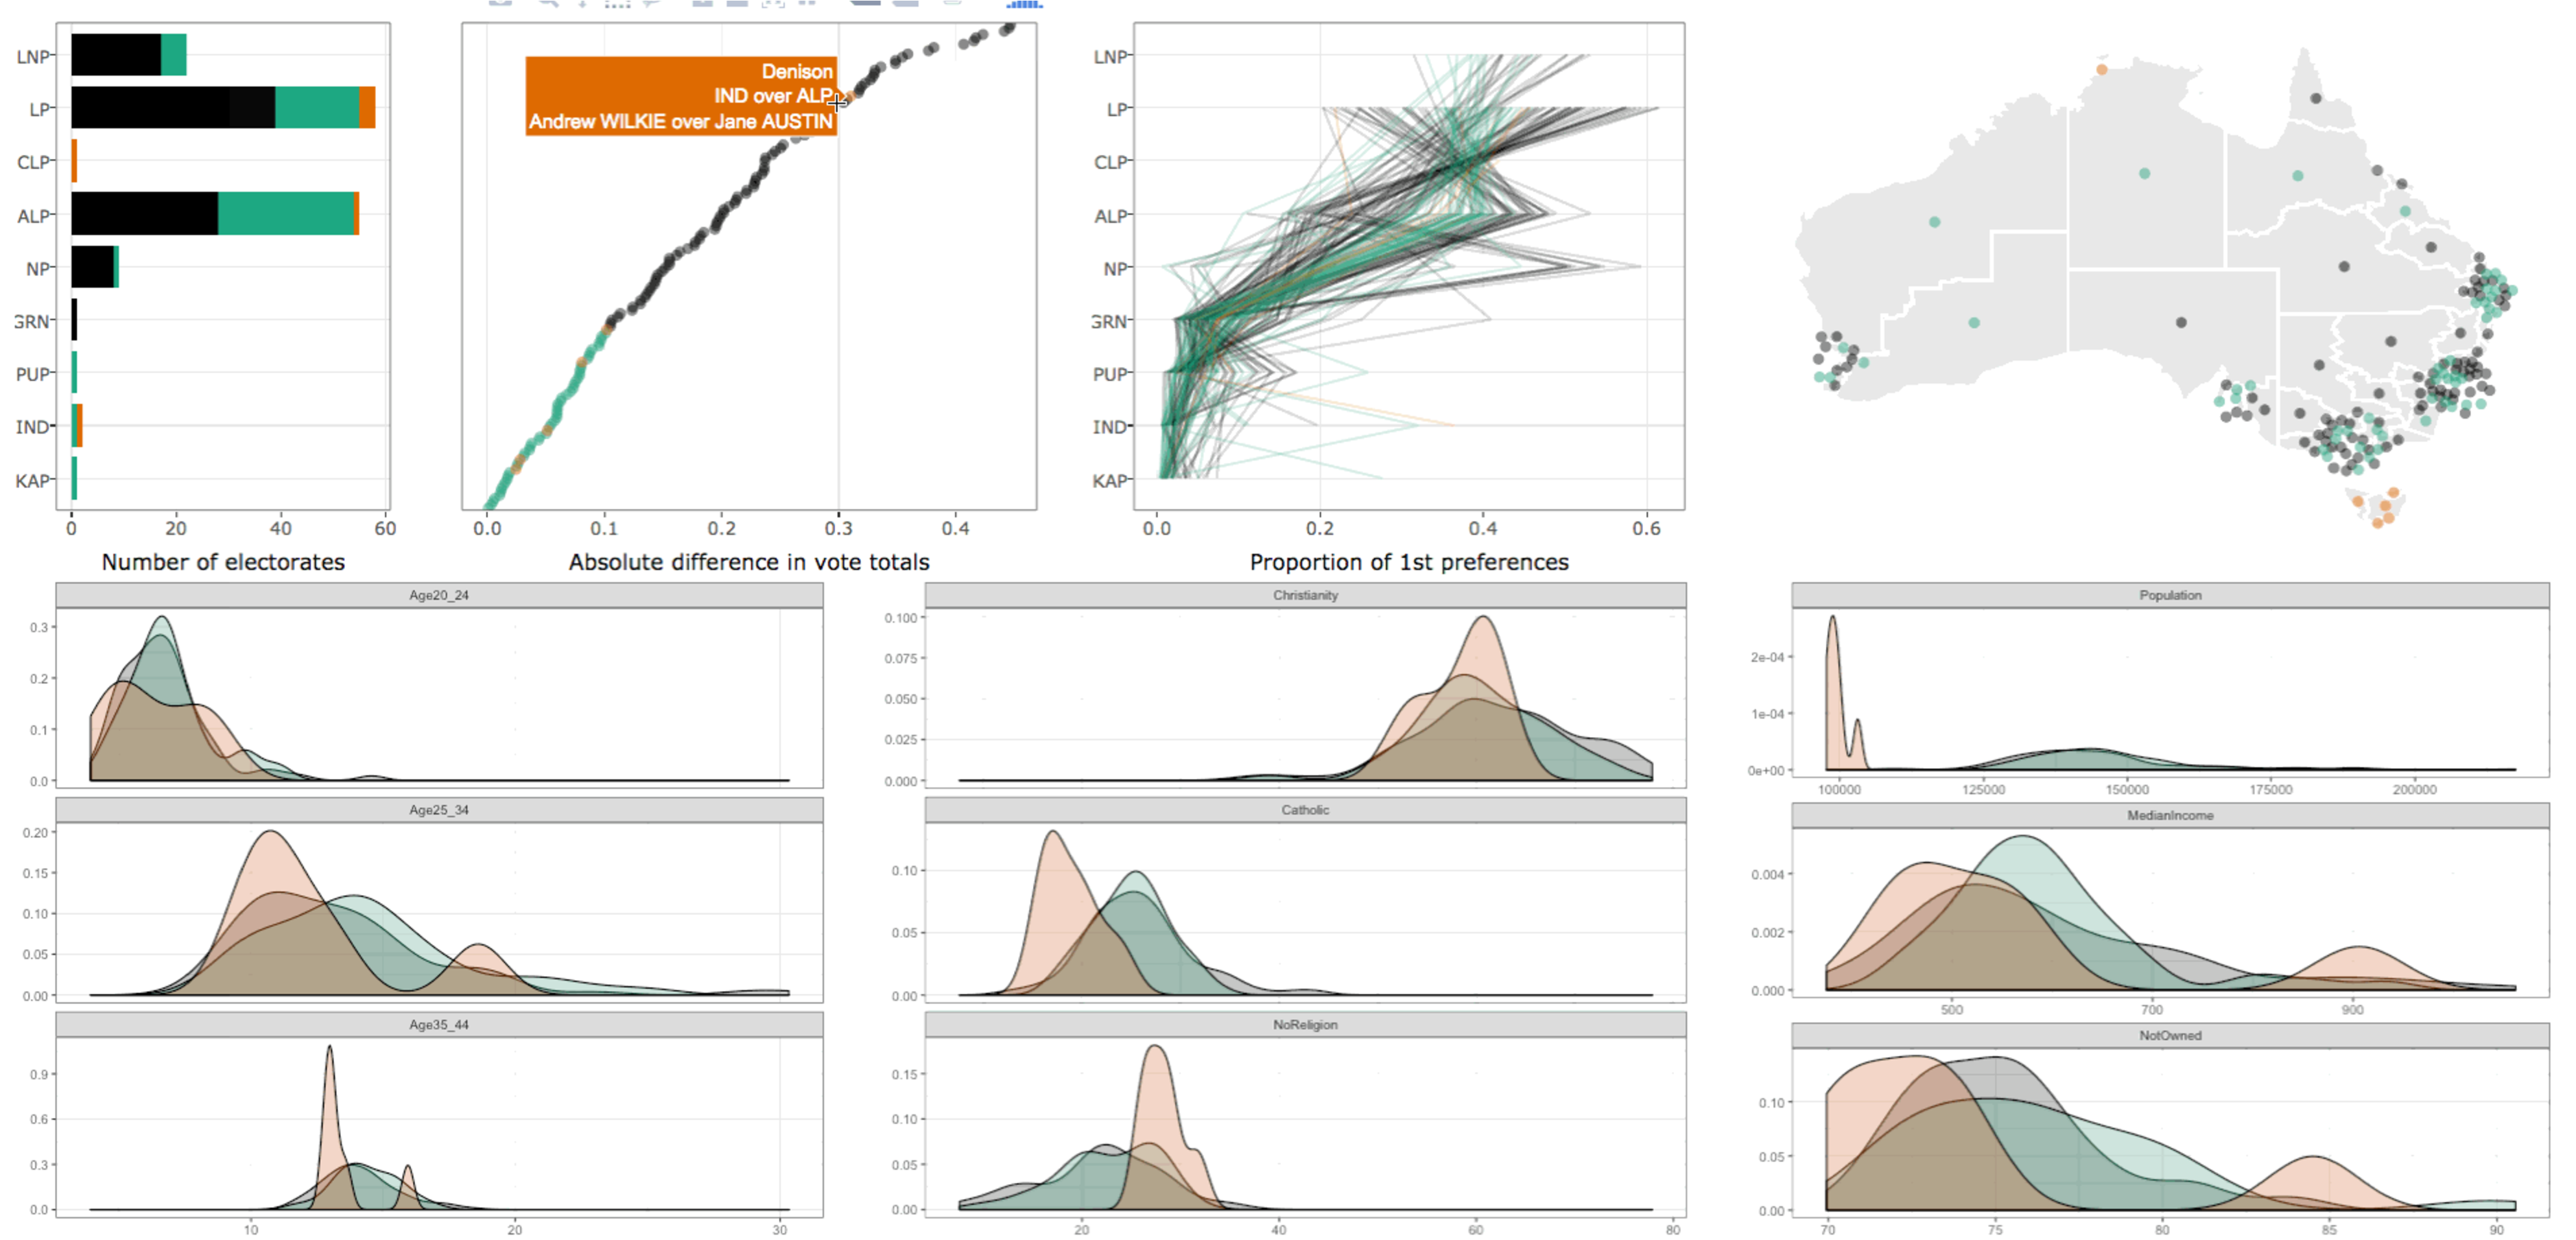
\includegraphics{images/eechidna-diff2.pdf}
\caption{\label{fig:eechidna-diff2}Electorates that experienced a close
election as well as electorates with small populations (in orange).}
\end{figure}

\section{Conclusion}\label{conclusion}

Interactive graphics, particularly multiple linked plots with support
for direct manipulation, provide a powerful data analysis tool for
posing queries and making comparisons. This paper gives three different
case studies applying interactive web graphics to real-world data sets
to extract insights and present the graphics themselves in an accessible
and convenient format. Furthermore, these graphical techniques can be
widely useful not only for the analyst conducting exploratory data
analysis, but also for understanding and diagnosing statistical models,
and presenting results to a wider audience.

Interactive web graphics are already widely used for presenting and
communicating results of an analysis (where the visualization type is
already known), but are less often used for exploring data -- mostly due
to a lack of tools for iteration within a larger statistical computing
environment. The \textbf{plotly} package aims to address this lack of
tools by enabling R users to produce highly interactive and dynamic web
graphics by leveraging already well-known and widely used interfaces for
exploratory data analysis. In particular, the \textbf{plotly} package
makes it easy to translate \textbf{ggplot2} graphics\footnote{Some
  recent estimates suggest that 100,000s of people use \textbf{ggplot2},
  a graphing interface which is especially well suited for creating
  exploratory graphics.} to a web-based version, and enable interactive
techniques such as highlighting and linked brushing (Wickham 2009).

All of the examples in the
\protect\hyperlink{exploring-pedestrian-counts}{exploring pedestrian
counts} section were created with \textbf{plotly} and are available as
standalone HTML files that can be easily deployed and shared with
well-established web technologies. The sections
\protect\hyperlink{tracking-disease-outbreak}{tracking disease outbreak}
and \protect\hyperlink{exploring-australian-election-data}{exploring
Australian election data} link \textbf{plotly} graphs using the
\textbf{shiny} package for authoring web applications to enable linked
interactions that compute statistical summaries based on graphical
queries defined by users. Furthermore, all of the examples across all of
these sections were created purely within R, and requires no knowledge
of web technologies such as HTML/JavaScript/CSS from the user. As a
result, projects such as \textbf{plotly} and \textbf{shiny} help
analysts focus on their primary task (data analysis) rather than the
implementation details typically involved when creating interactive web
graphics.

\section*{References}

\hypertarget{refs}{}
\hypertarget{ref-grand-tour}{}
Asimov, Daniel. 1985. ``The Grand Tour: A Tool for Viewing
Multidimensional Data.'' \emph{SIAM J. Sci. Stat. Comput.} 6 (1).
Philadelphia, PA, USA: Society for Industrial; Applied Mathematics:
128--43. doi:\href{https://doi.org/10.1137/0906011}{10.1137/0906011}.

\hypertarget{ref-Buja:1991vh}{}
Buja, Andreas, John Alan McDonald, John Michalak, and Werner Stuetzle.
1991. ``Interactive data visualization using focusing and linking.''
\emph{IEEE Proceedings of Visualization}, February, 1--8.

\hypertarget{ref-brushing-pcp}{}
Carr, Wegman, D. B. 1996. ``ExplorN: Design Considerations Past and
Present.'' Fairfax, VA: Center for Computational Statistics, George
Mason University.

\hypertarget{ref-shiny}{}
Chang, Winston, Joe Cheng, JJ Allaire, Yihui Xie, and Jonathan
McPherson. 2015. \emph{shiny: Web Application Framework for R}. R
package version 0.12.2. \url{http://CRAN.R-project.org/package=shiny}.

\hypertarget{ref-leaflet}{}
Cheng, Joe, and Yihui Xie. 2015. \emph{leaflet: Create Interactive Web
Maps with the JavaScript 'Leaflet' Library}. R package version
1.0.0.9999. \url{http://rstudio.github.io/leaflet/}.

\hypertarget{ref-eechidna}{}
Cook, Di, Heike Hofmann, Rob Hyndman, Thomas Lumley, Ben Marwick, Carson
Sievert, Nicholas Tierney, Nathaniel Tomasetti, and Fang Zhou. 2016.
\emph{eechidna: Exploring Election and Census Highly Informative Data
Nationally for Australia}. R package version 0.1.
\url{https://github.com/ropenscilabs/eechidna}.

\hypertarget{ref-ggobi:2007}{}
Cook, Dianne, and Deborah F. Swayne. 2007. \emph{Interactive and Dynamic
Graphics for Data Analysis : With R and GGobi}. Use R ! New York:
Springer. \url{http://www.ggobi.org/book/}.

\hypertarget{ref-Cook:2007uk}{}
Cook, Dianne, Andreas Buja, and Deborah F Swayne. 1996. ``Interactive
High-Dimensional Data Visualization.'' \emph{Journal of Computational
and Graphical Statistics}, December, 1--23.

\hypertarget{ref-anomalous}{}
Hyndman, Rob J, Earo Wang, and Nikolay Laptev. 2016. \emph{anomalous:
Unusual Time Series Detection}. R package version 0.1.0.

\hypertarget{ref-Inselberg:85}{}
Inselberg, Alfred. 1985. ``The Plane with Parallel Coordinates.''
\emph{Visual Computer} 1 (4): 69--91.
doi:\href{https://doi.org/10.1007/BF01898350}{10.1007/BF01898350}.

\hypertarget{ref-zika-nyt}{}
McNeil, Donald G., and Daniel Victor. 2016. ``First U.s. Death Tied to
Zika Is Reported in Puerto Rico.''
\url{http://www.nytimes.com/2016/04/30/health/zika-virus-first-death-in-us-puerto-rico.html}.

\hypertarget{ref-melbourne}{}
Melbourne, City of. 2016. ``City of Melbourne's Open Data Platform.''
\url{https://data.melbourne.vic.gov.au/}.

\hypertarget{ref-RCore}{}
R Core Team. 2016. \emph{R: A Language and Environment for Statistical
Computing}. Vienna, Austria: R Foundation for Statistical Computing.
\url{http://www.R-project.org/}.

\hypertarget{ref-stl}{}
R. B. Cleveland, J.E. McRae, W. S. Cleveland, and I. Terpenning. 1990.
``STL: A Seasonal-Trend Decomposition Procedure Based on Loess.''
\emph{Journal of Official Statistics}, no. 6: 3--73.

\hypertarget{ref-zika-data}{}
Rodriguez, Dania M., Michael A Johansson, moiradillon2, Luis
Mier-y-Teran-Romero, eyq9, YoJimboDurant, Aash Anand, et al. 2016.
``Zika: September 7, 2016.''
doi:\href{https://doi.org/10.5281/zenodo.61753}{10.5281/zenodo.61753}.

\hypertarget{ref-pedestrians}{}
Sievert, Carson. 2016a. \emph{pedestrians: Tools for Exploring
Melbourne's Pedestrian Data}. R package version 0.0.1.
\url{https://github.com/cpsievert/pedestrians}.

\hypertarget{ref-plotly-book}{}
---------. 2016b. ``Plotly for R.''
\url{https://cpsievert.github.io/plotly_book}.

\hypertarget{ref-zikar}{}
---------. 2016c. \emph{zikar: Tools for exploring publicly available
Zika data}. R package version 0.0.0.9000.

\hypertarget{ref-plotly}{}
Sievert, Carson, Chris Parmer, Toby Hocking, Scott Chamberlain, Karthik
Ram, Marianne Corvellec, and Pedro Despouy. 2016. \emph{plotly: Create
Interactive Web Graphics via 'plotly.js'}. R package version 4.5.6.9000.
\url{https://CRAN.R-project.org/package=plotly}.

\hypertarget{ref-xgobi}{}
Swayne, Deborah F, Dianne Cook, and Andreas Buja. 1998. ``XGobi:
Interactive Dynamic Data Visualization in the X Window System.''
\emph{Journal of Computational and Graphical Statistics} 7 (1): 113--30.

\hypertarget{ref-MANET}{}
Unwin A., Hofmann H., Hawkins G. 1996. ``Interactive Graphics for Data
Sets with Missing Values - Manet.'' \emph{Journal of Computational and
Graphical Statistics} 4 (6).

\hypertarget{ref-tscognostics}{}
Wang, Earo. 2016. \emph{tscognostics: Time Series Cognostics}. R package
version 0.0.1. \url{https://github.com/earowang/tscognostics}.

\hypertarget{ref-Wegman:90}{}
Wegman, E.J. 1990. ``Hyperdimensional Data Analysis Using Parallel
Coordinates,'' no. 85: 664--75.

\hypertarget{ref-ggplot2}{}
Wickham, Hadley. 2009. \emph{ggplot2: Elegant Graphics for Data
Analysis}. Springer-Verlag New York. \url{http://ggplot2.org}.

\hypertarget{ref-model-vis-paper}{}
Wickham, Hadley, Dianne Cook, and Heike Hofmann. 2015. ``Visualizing
Statistical Models: Removing the Blindfold.'' \emph{Statistical Analysis
and Data Mining: The ASA Data Science Journal} 8 (4): 203--25.

\hypertarget{ref-mgcv}{}
Wood, S.N. 2006. \emph{Generalized Additive Models: An Introduction with
R}. Chapman; Hall/CRC.



\end{document}
